\chapter{Experiment}
\section{Slab Waveguide}
Using the software RSoft a slab waveguide should be designed. The chosen material is glass with a refractive index $n$~=~1.44 and a width 2.5~$\upmu$m.  The input parameters were the following:
\begin{itemize}
	\item Width: 2.5
uau..u.��.��			ee	errer__r_cc_cw
	\item index difference: 0.44
	\item background index: 1
 \end{itemize}



In Figure \ref{fig:1_index} the resulted index profile can be seen.
\begin{figure}[h]%
\centering
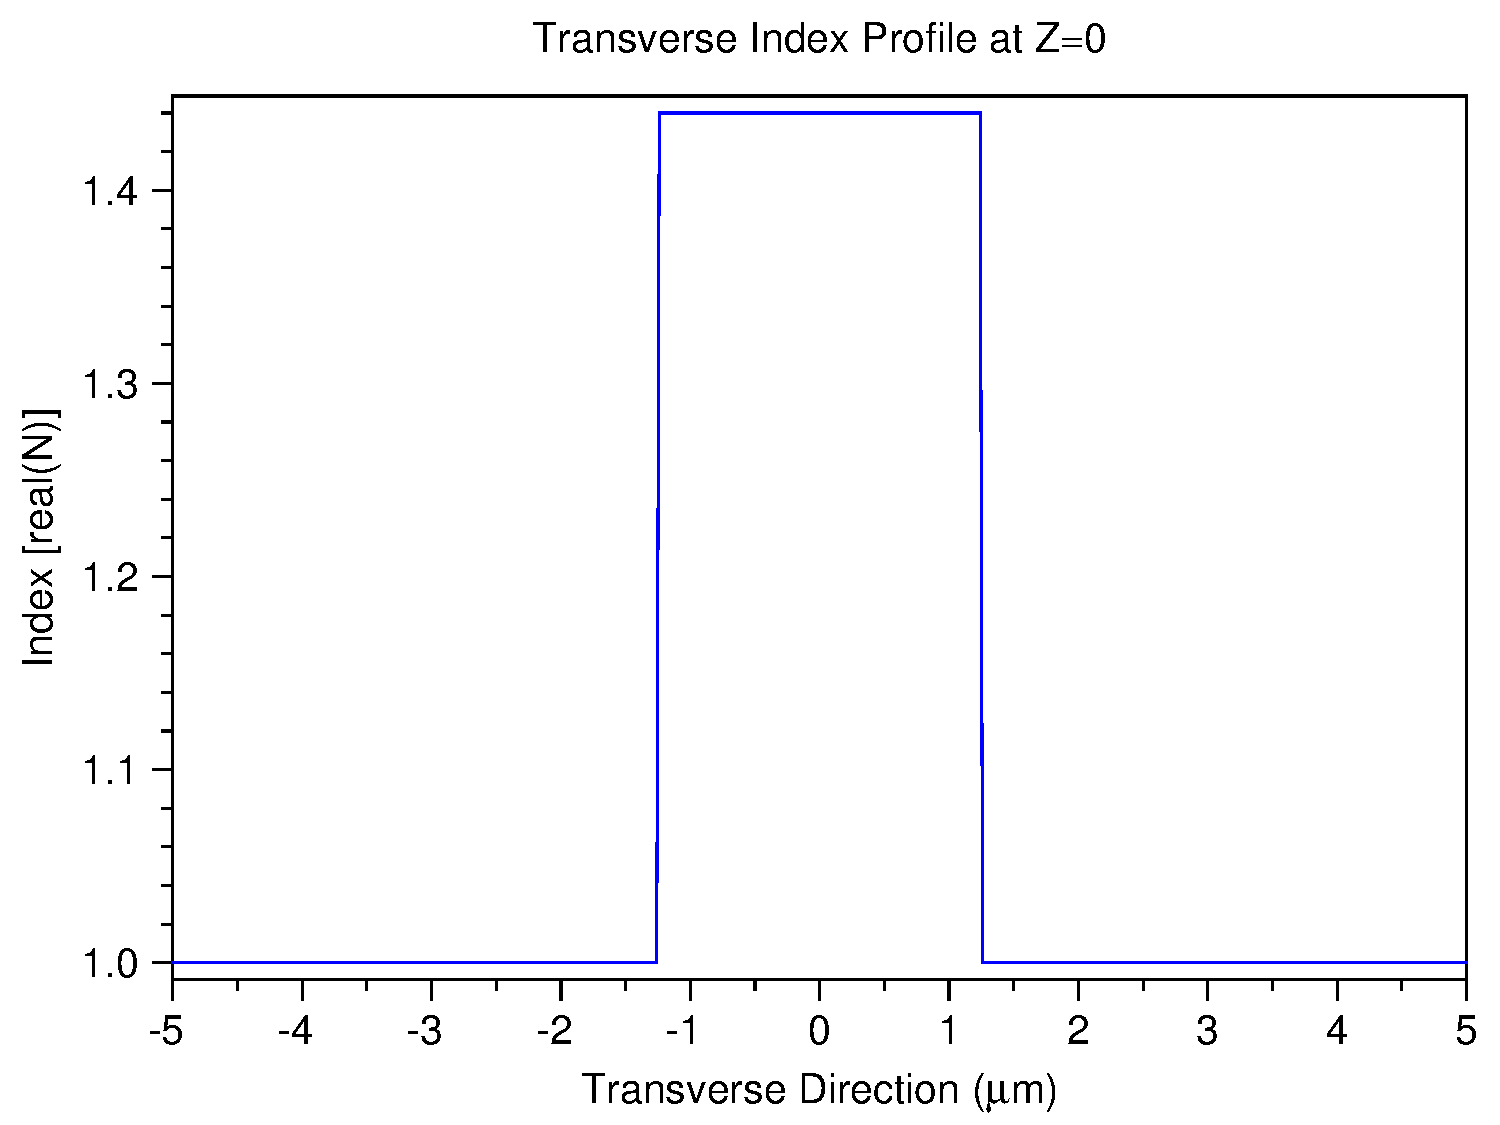
\includegraphics[totalheight=5.5 cm]{Grafiken/1_index.pdf}%
����\\\tt\t{{t{ee{errerllrlfflfeefe
\label{fig:1_index}%
\end{figure}

After moving the excitation point outside the waveguide core and running a simulation for the field distribution the following results came out (cf. figure \ref{fig:1_TE}).

\begin{figure}[h]%
\centering
%\begin{adjustwidth}{0cm}{0cm}
	\subfloat[TE00]{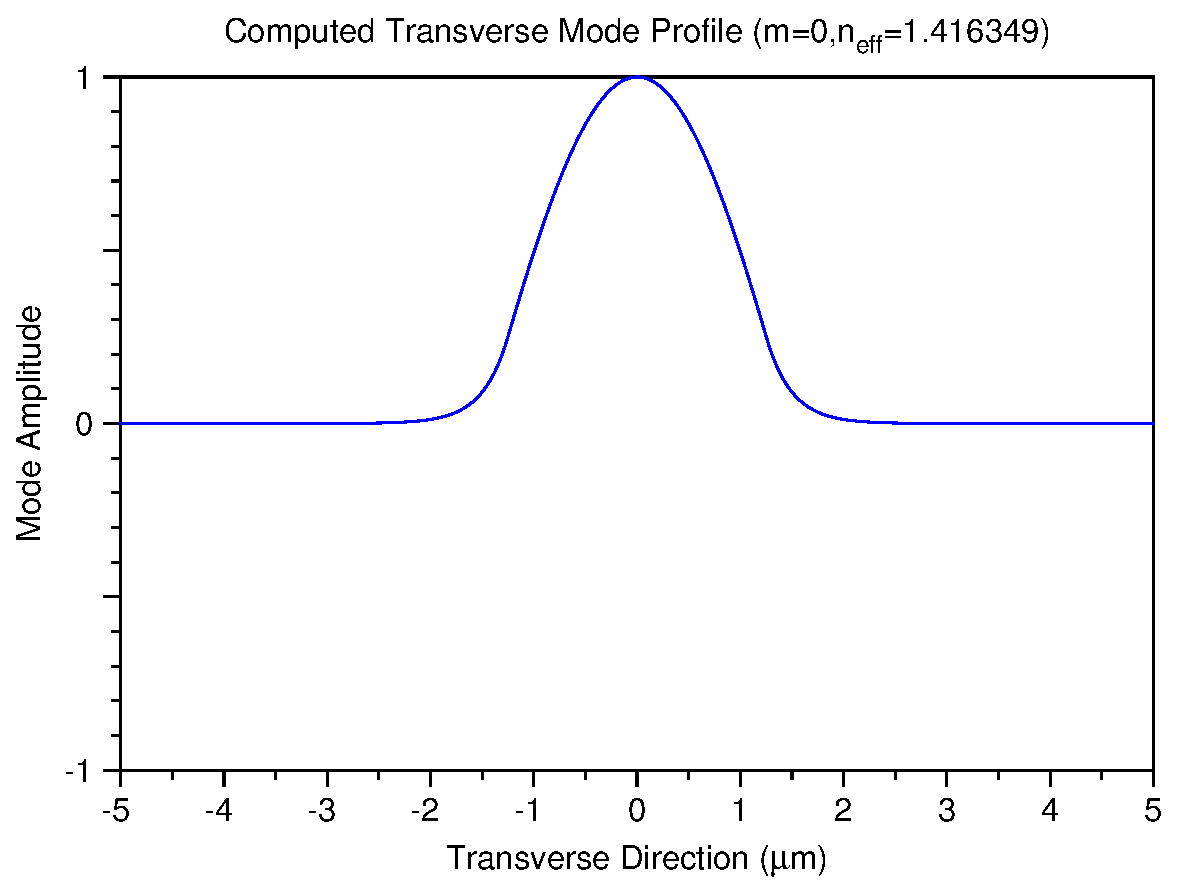
\includegraphics[totalheight=4.5 cm]{Grafiken/modes_TE00.pdf}\label{fig:1_TE00}}
	\subfloat[TE01]{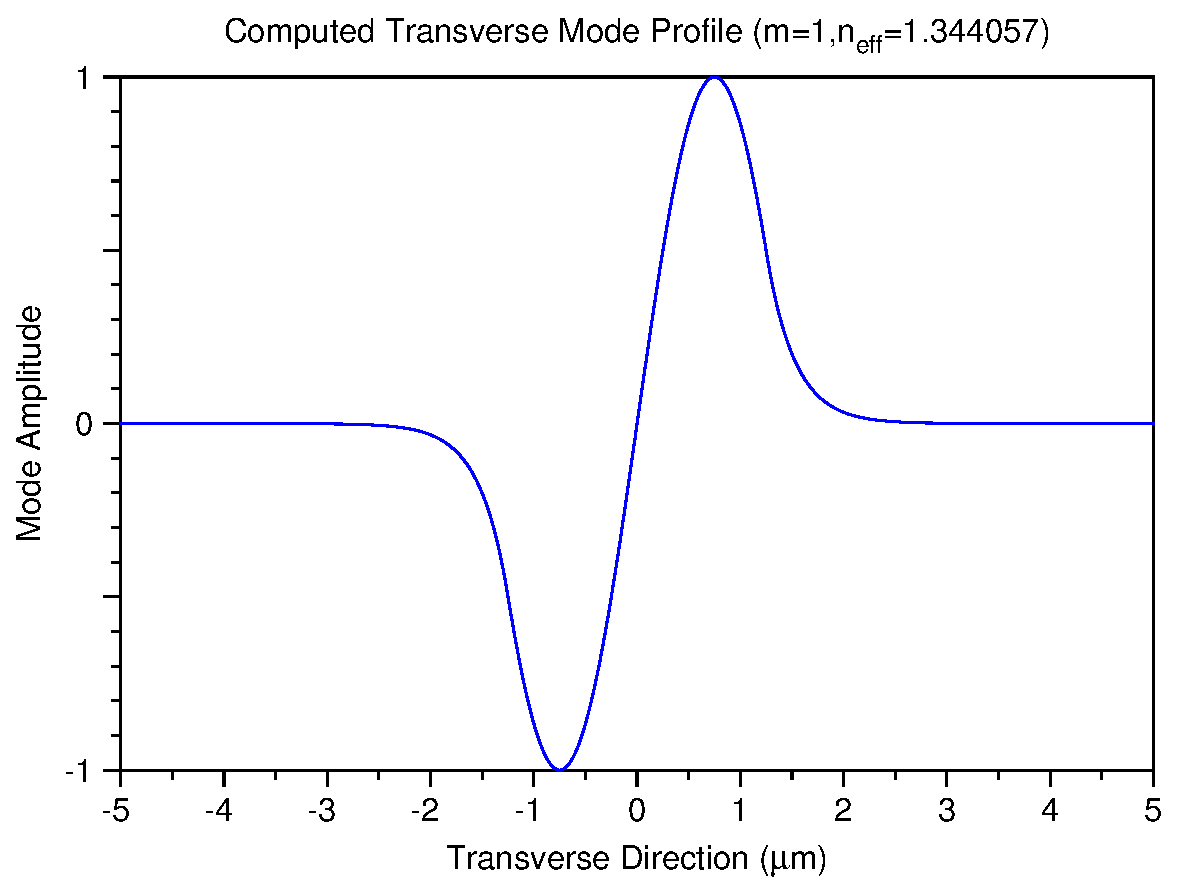
\includegraphics[totalheight=4.5 cm]{Grafiken/modes_TE01.pdf} \label{fig:1_TE01}}\\
		\subfloat[TE02]{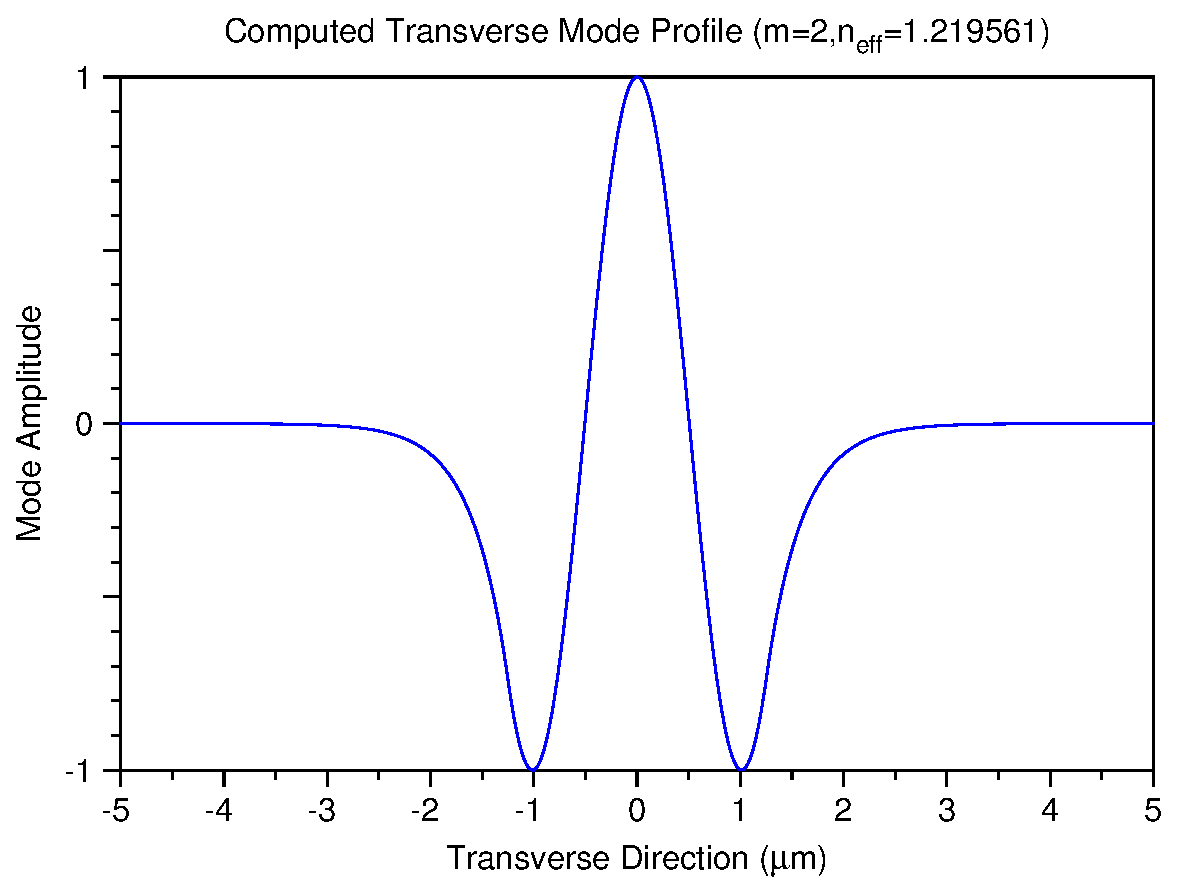
\includegraphics[totalheight=4.5 cm]{Grafiken/modes_TE02.pdf}\label{fig:1_TE02}}
	\subfloat[TE03]{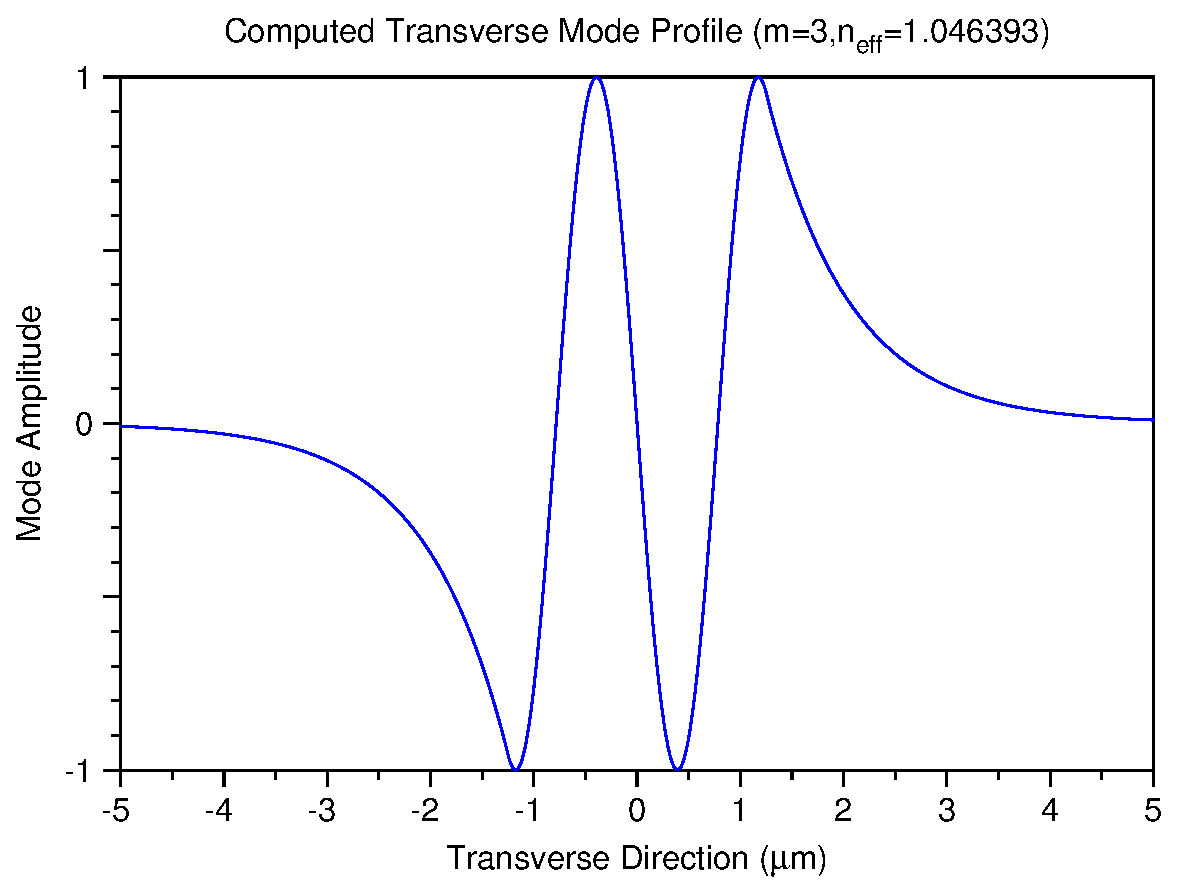
\includegraphics[totalheight=4.5 cm]{Grafiken/modes_TE03.pdf} \label{fig:1_TE03}}
\caption{Calculated TE modes.}%
\label{fig:1_TE}%
\end{figure}

\newpage
As in figure \ref{fig:1_TE} seen there are four different modes available, namely m=0,1,2 and 3. As the E-field is continuous in the transverse direction no kinks are seen.  For the m=3 the refractive index is almost to 1 (air), so it can be concluded that this is the last mode for this waveguide at this frequency.\\
The results of the TM simulation shown in figure \ref{fig:1_TM1} were also not surprising.

\begin{figure}[h]%
\centering
%\begin{adjustwidth}{0cm}{0cm}
	\subfloat[TM00]{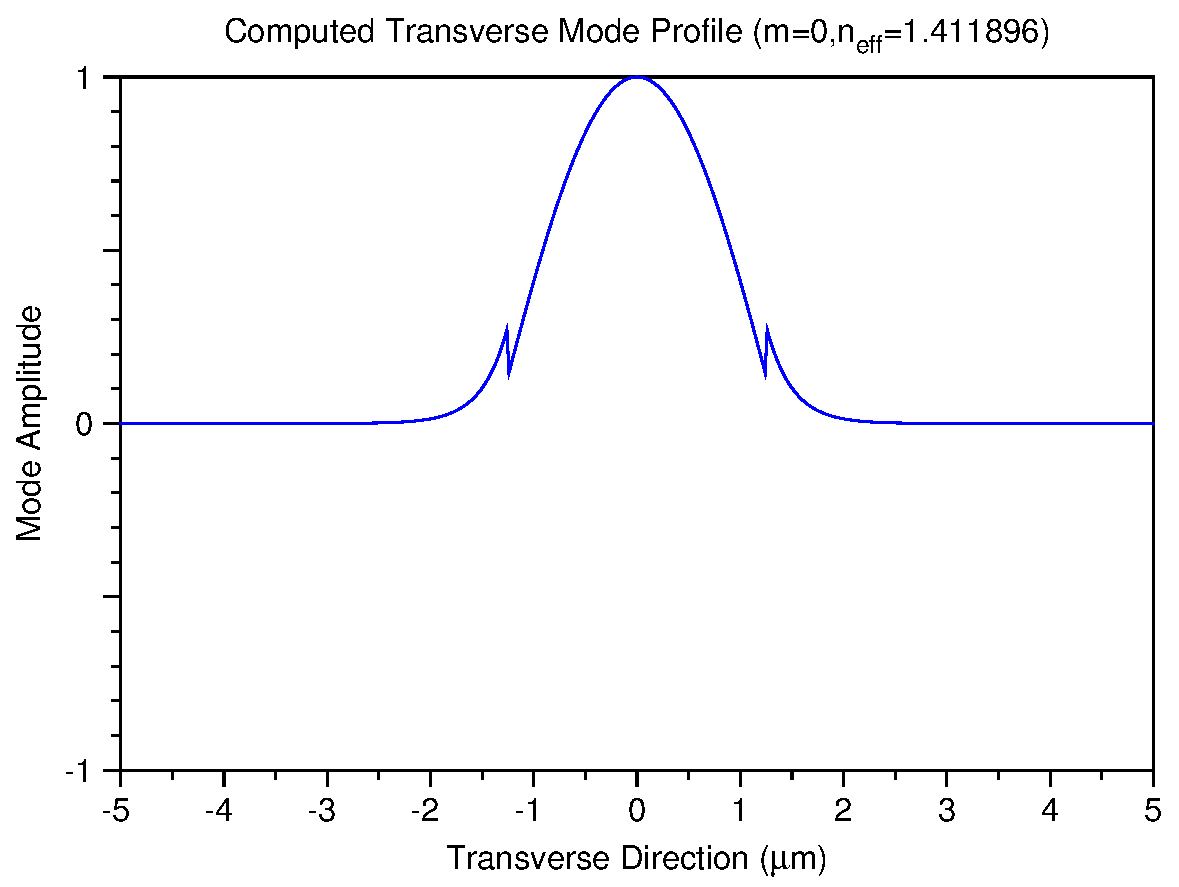
\includegraphics[totalheight=4.5 cm]{Grafiken/modes_TM00.pdf}\label{fig:1_TM00}}
	\subfloat[TM01]{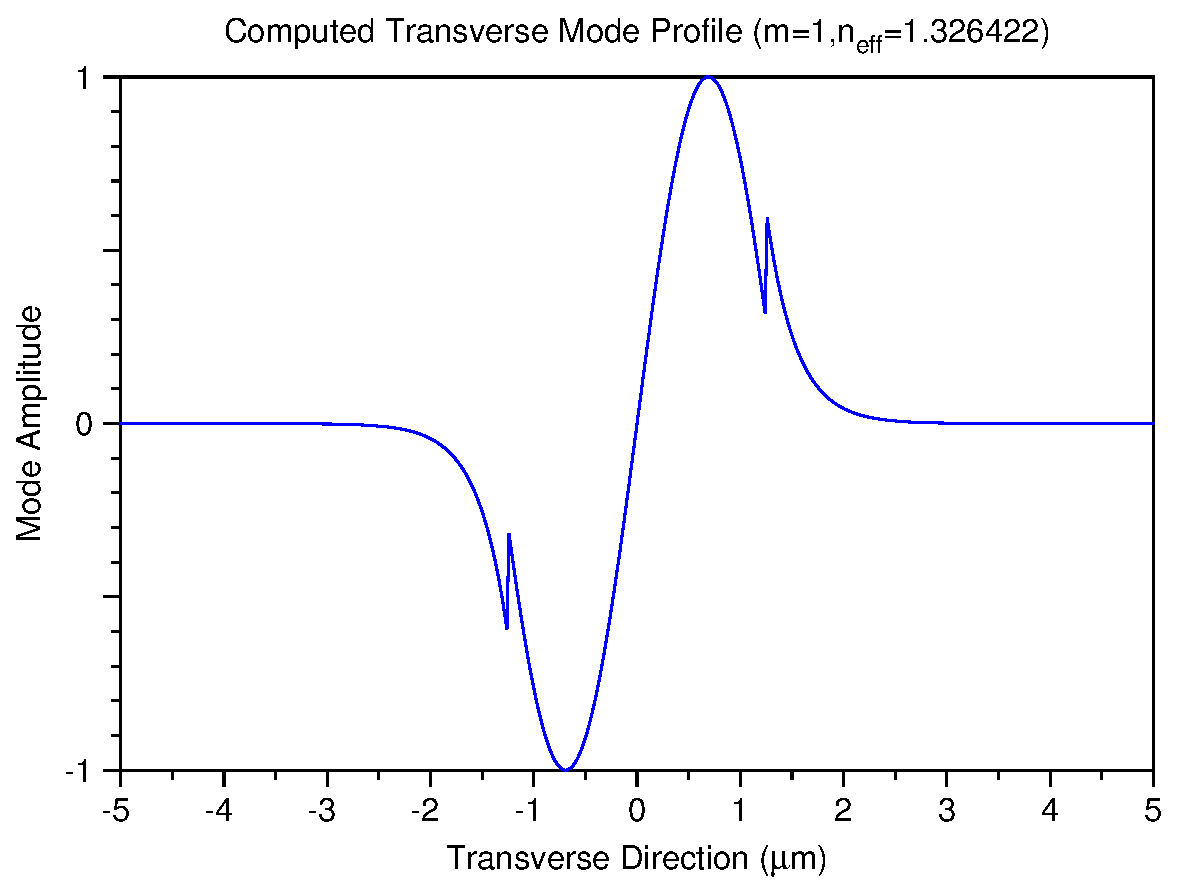
\includegraphics[totalheight=4.5 cm]{Grafiken/modes_TM01.pdf} \label{fig:1_TM01}}\\
\caption{Calculated TM modes.}%
\label{fig:1_TM1}%
\end{figure}

\begin{figure}[h]%
\centering
%\begin{adjustwidth}{0cm}{0cm}
		\subfloat[TM02]{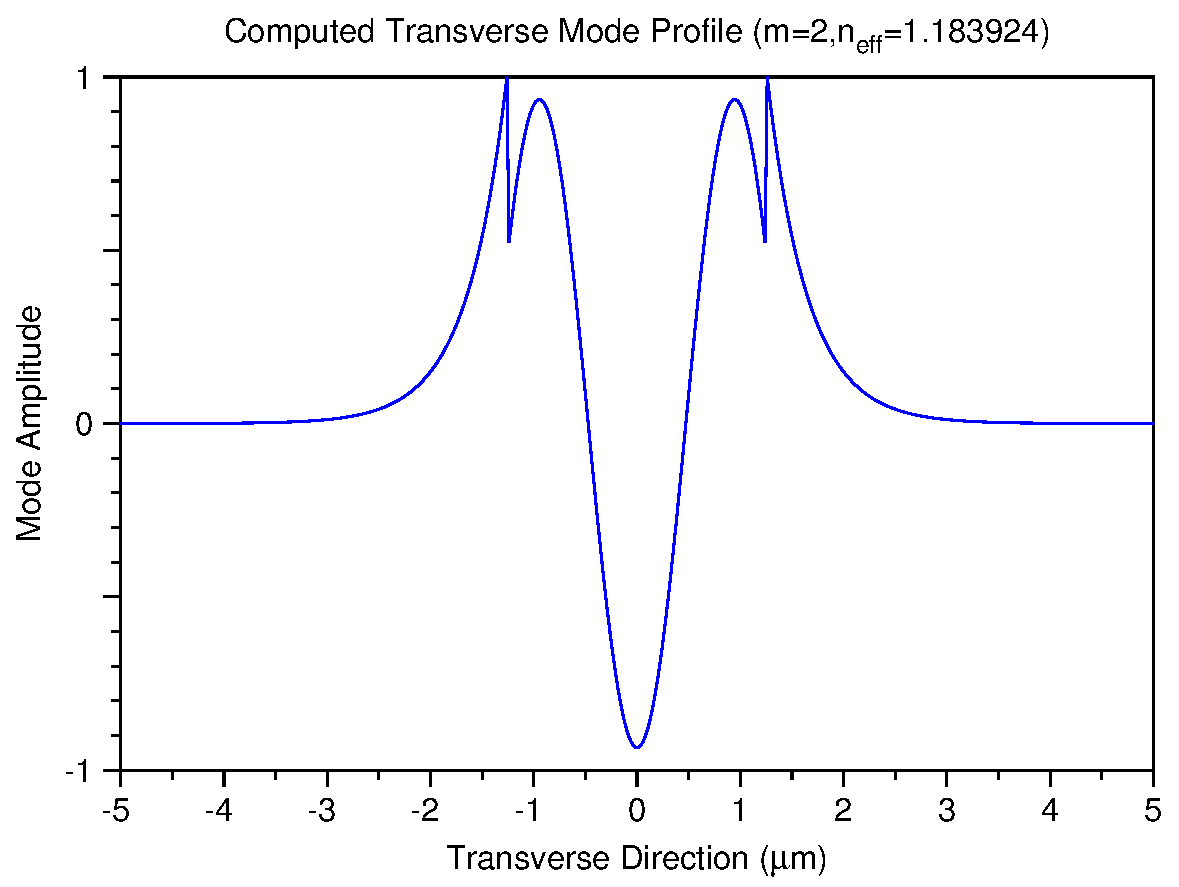
\includegraphics[totalheight=4.5 cm]{Grafiken/modes_TM02.pdf}\label{fig:1_TM02}}
	\subfloat[TM03]{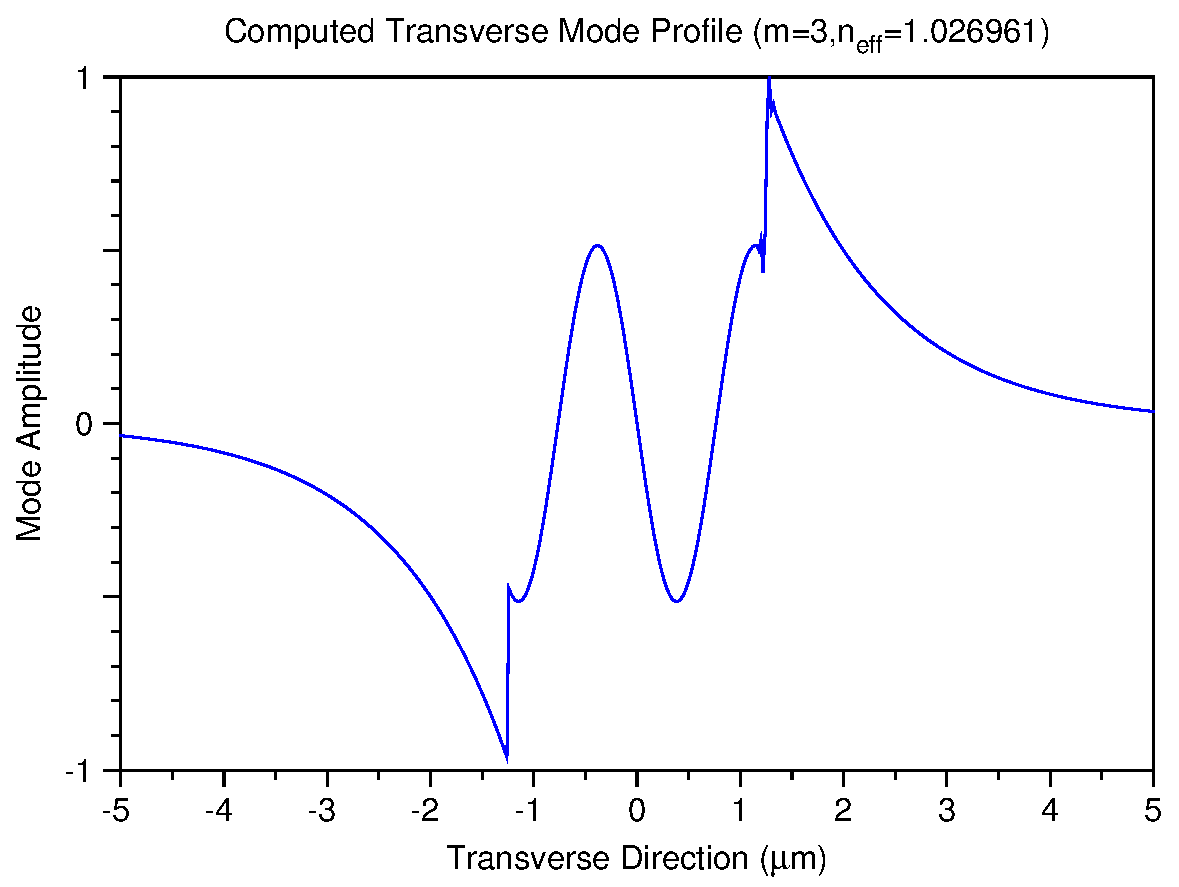
\includegraphics[totalheight=4.5 cm]{Grafiken/modes_TM03.pdf} \label{fig:1_TM03}}
\caption{Calculated TM modes.}%
\label{fig:1_TM2}%
\end{figure}
\newpage
Again four modes are available.

The kinks are a result of the discontinuity of $\vec{\mathrm{H}}$ field on the boundary.
After reducing the wavelength (increasing the frequency) the waveguide can accept even more modes. This applies for TE and TM modes. As a proof a wavelength of 0.7~$\upmu$m is chosen and the simulation is repeated (cf. fig \ref{fig:1_0307}).

\begin{figure}[h]%
\centering
%\begin{adjustwidth}{0cm}{0cm}
	\subfloat[TE03]{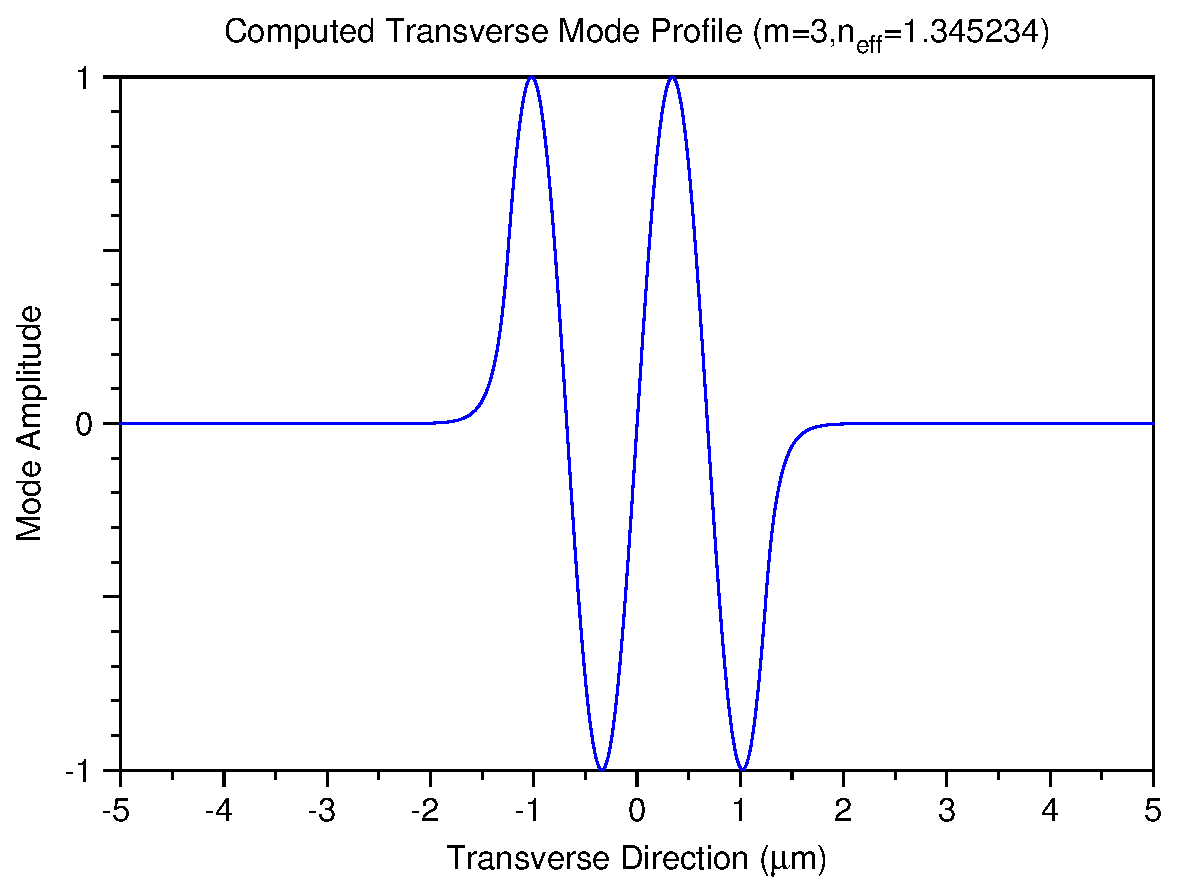
\includegraphics[totalheight=4.5 cm]{Grafiken/modes_TE_0_7_03.pdf}\label{fig:1_TE03}}
	\subfloat[TM03]{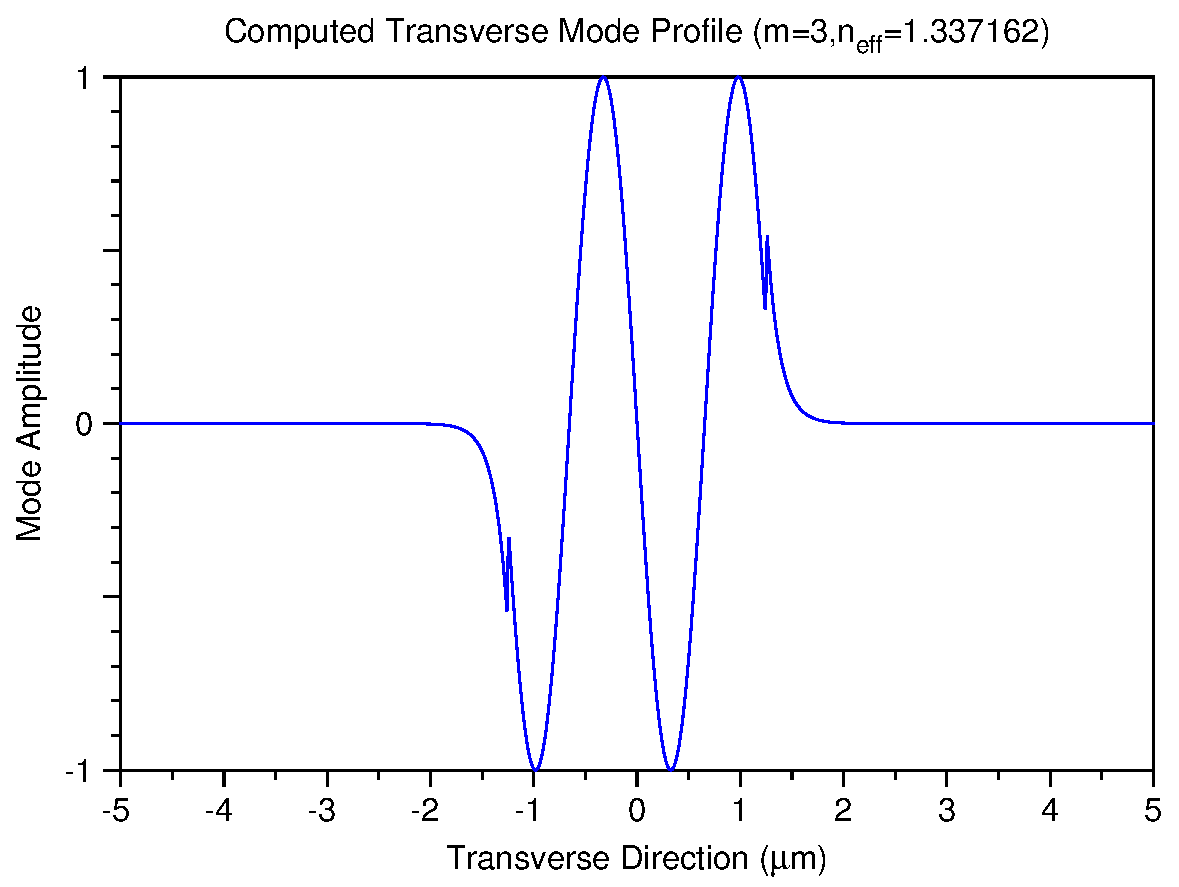
\includegraphics[totalheight=4.5 cm]{Grafiken/modes_TM_0_7_03.pdf} \label{fig:1_TM03}}\\
		\subfloat[TE07]{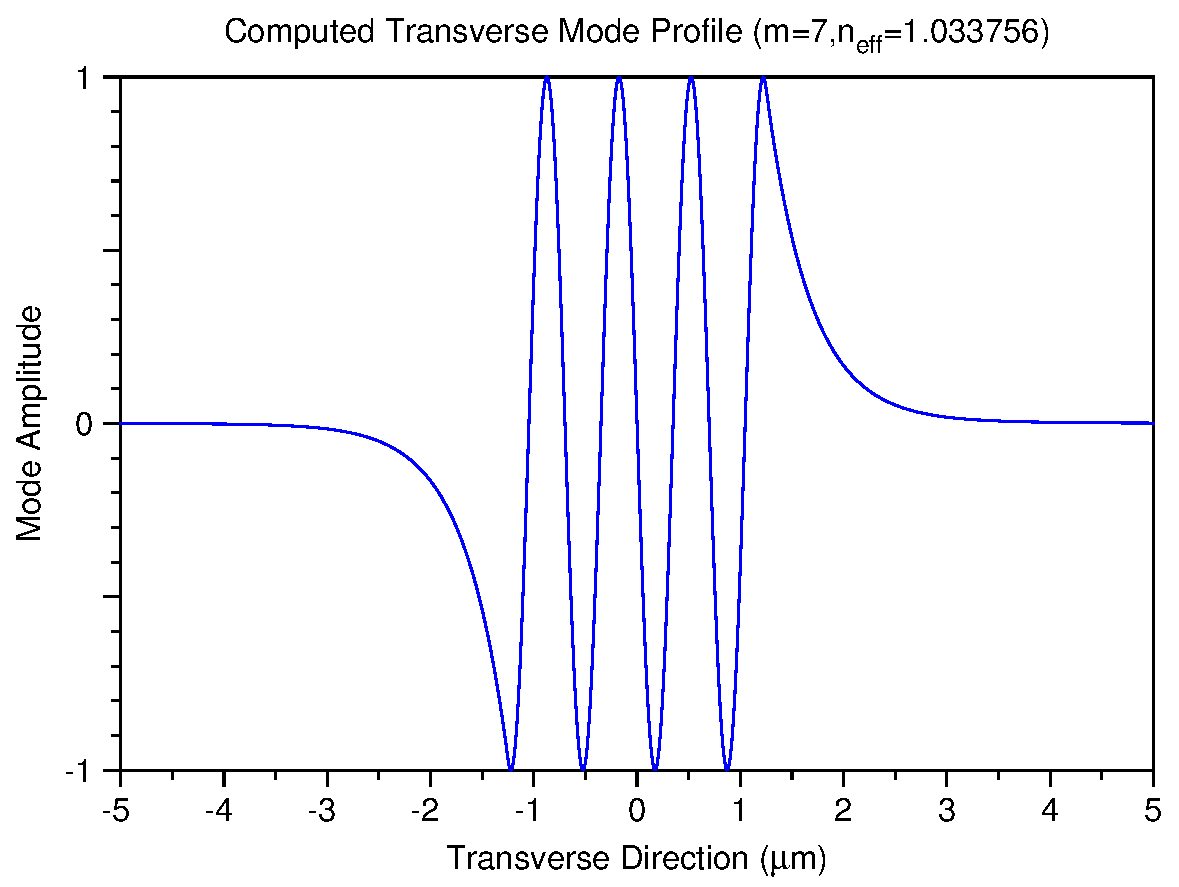
\includegraphics[totalheight=4.5 cm]{Grafiken/modes_TE_0_7_07.pdf}\label{fig:1_TE07}}
	\subfloat[TM07]{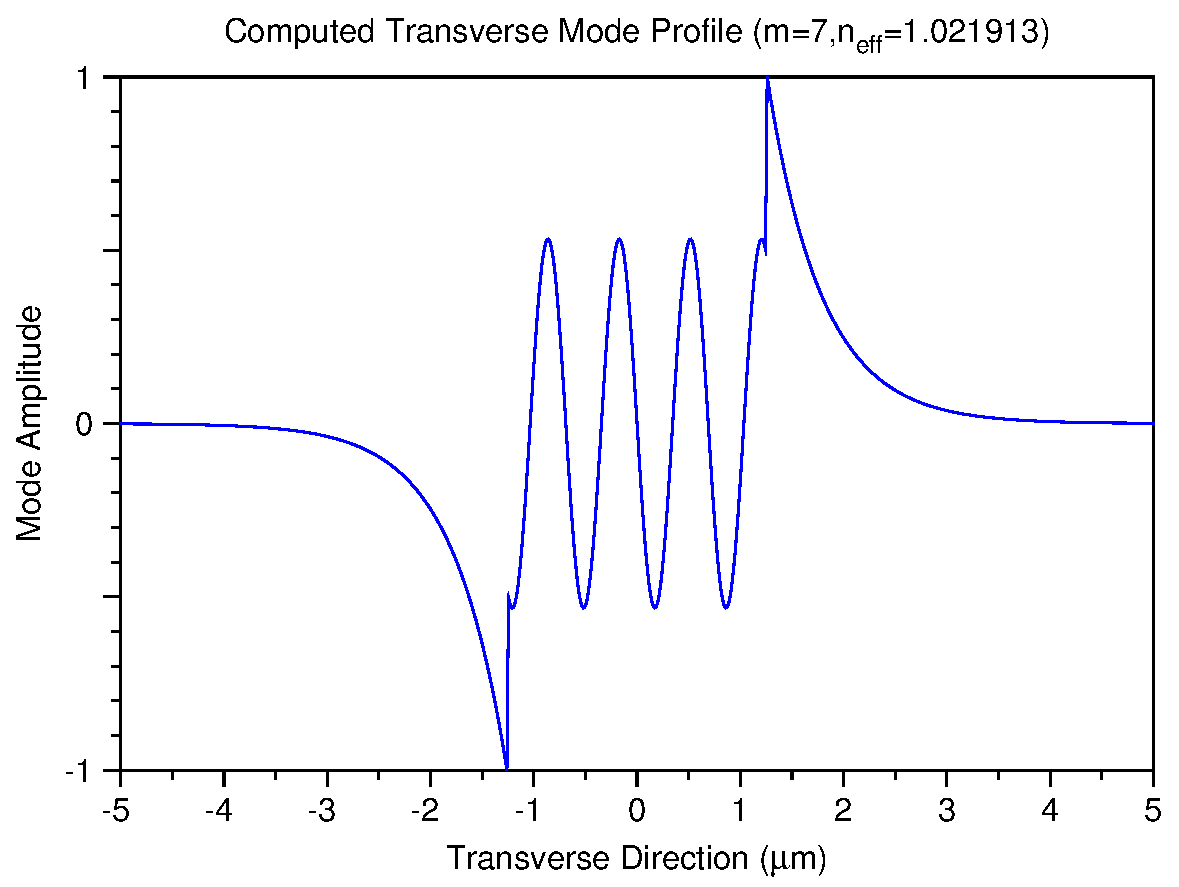
\includegraphics[totalheight=4.5 cm]{Grafiken/modes_TM_0_7_07.pdf} \label{fig:1_TM07}}
\caption{Modes at $\lambda = 0.7~\upmu$m.}%
\label{fig:1_0307}%
\end{figure}

At this wavelength there are already 8 different modes available. As seen from the diagram the steeper curves show that the fields are also better confined. To mention is also the better confinement of the TE modes than the one of the TM modes.
After increasing the wavelength to 2.0~$\upmu$m (150 THz) results in fewer modes ($m \leq 3$)(for TE and TM). Furthermore they are worse confined to the waveguide core (cf. fig \ref{fig:1_2_02}).


\begin{figure}[h]%
\centering
%\begin{adjustwidth}{0cm}{0cm}
	\subfloat[TE02]{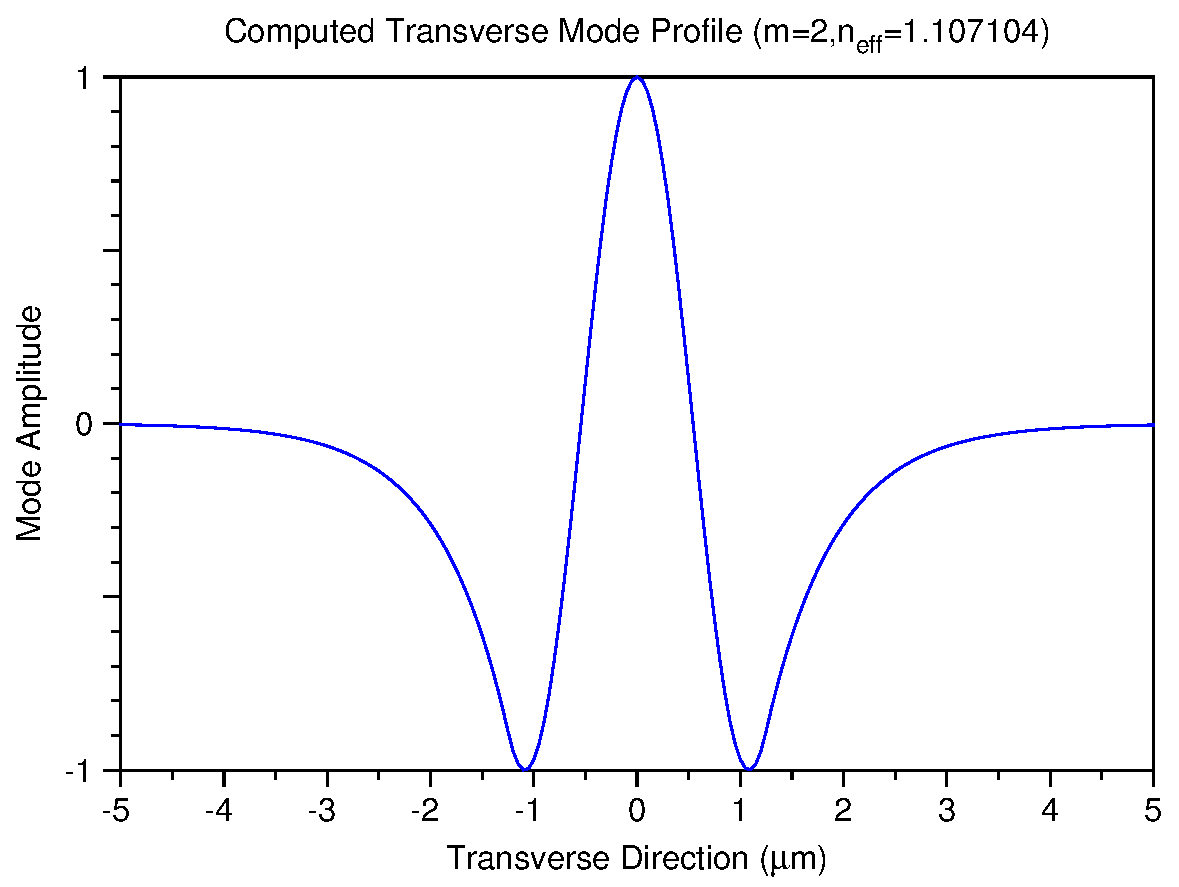
\includegraphics[totalheight=4.5 cm]{Grafiken/modes_TE_2_0_02.pdf}\label{fig:1_TE02_2}}
	\subfloat[TM02]{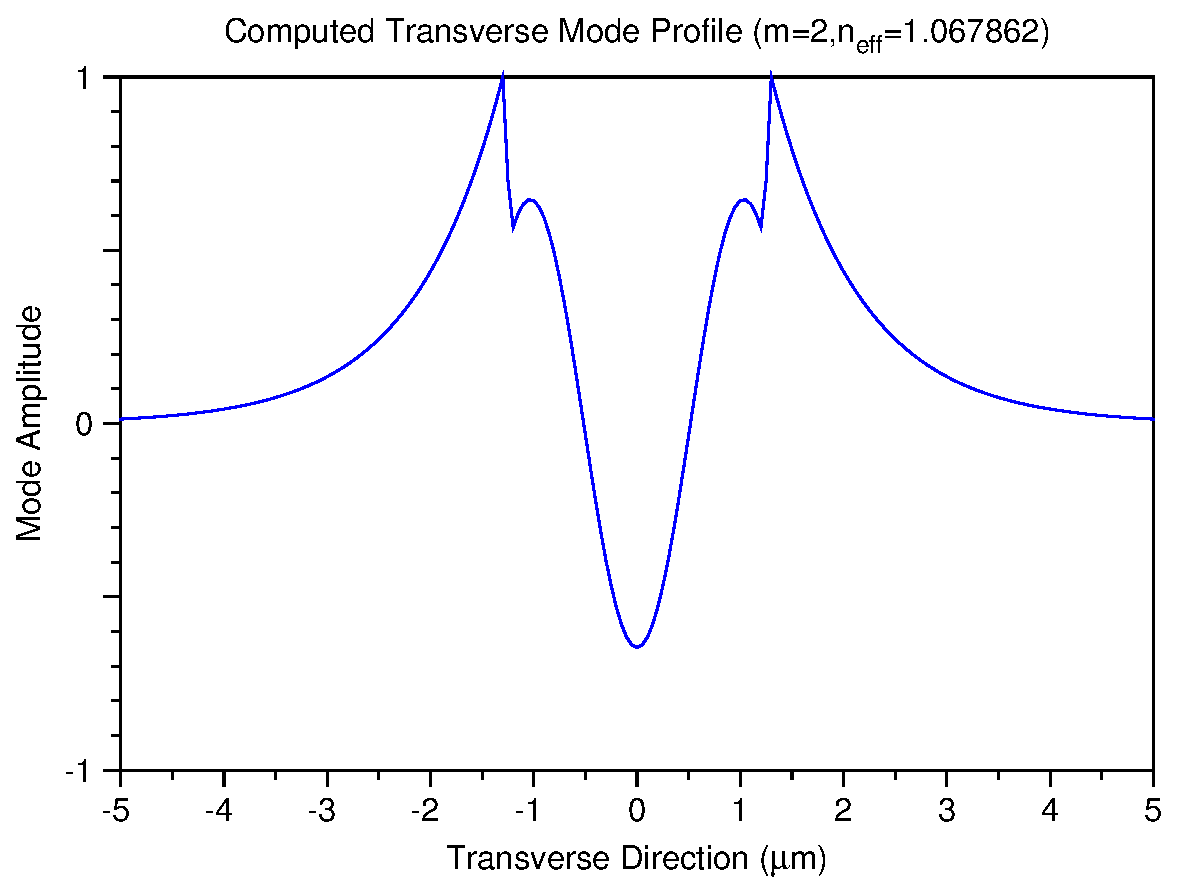
\includegraphics[totalheight=4.5 cm]{Grafiken/modes_TM_2_0_02.pdf} \label{fig:1_TM02_2}}
\caption{Modes at $\lambda = 2.0~\upmu$m.}%
\label{fig:1_2_02}%
\end{figure}

Effective Index:

For calculating the effective refractive index neff a scan with a "sweep" of the frequency was performed. The results are shown in figure \ref{fig:1_neff}.

\begin{figure}[h]%
\centering
%\begin{adjustwidth}{0cm}{0cm}
	\subfloat[TE]{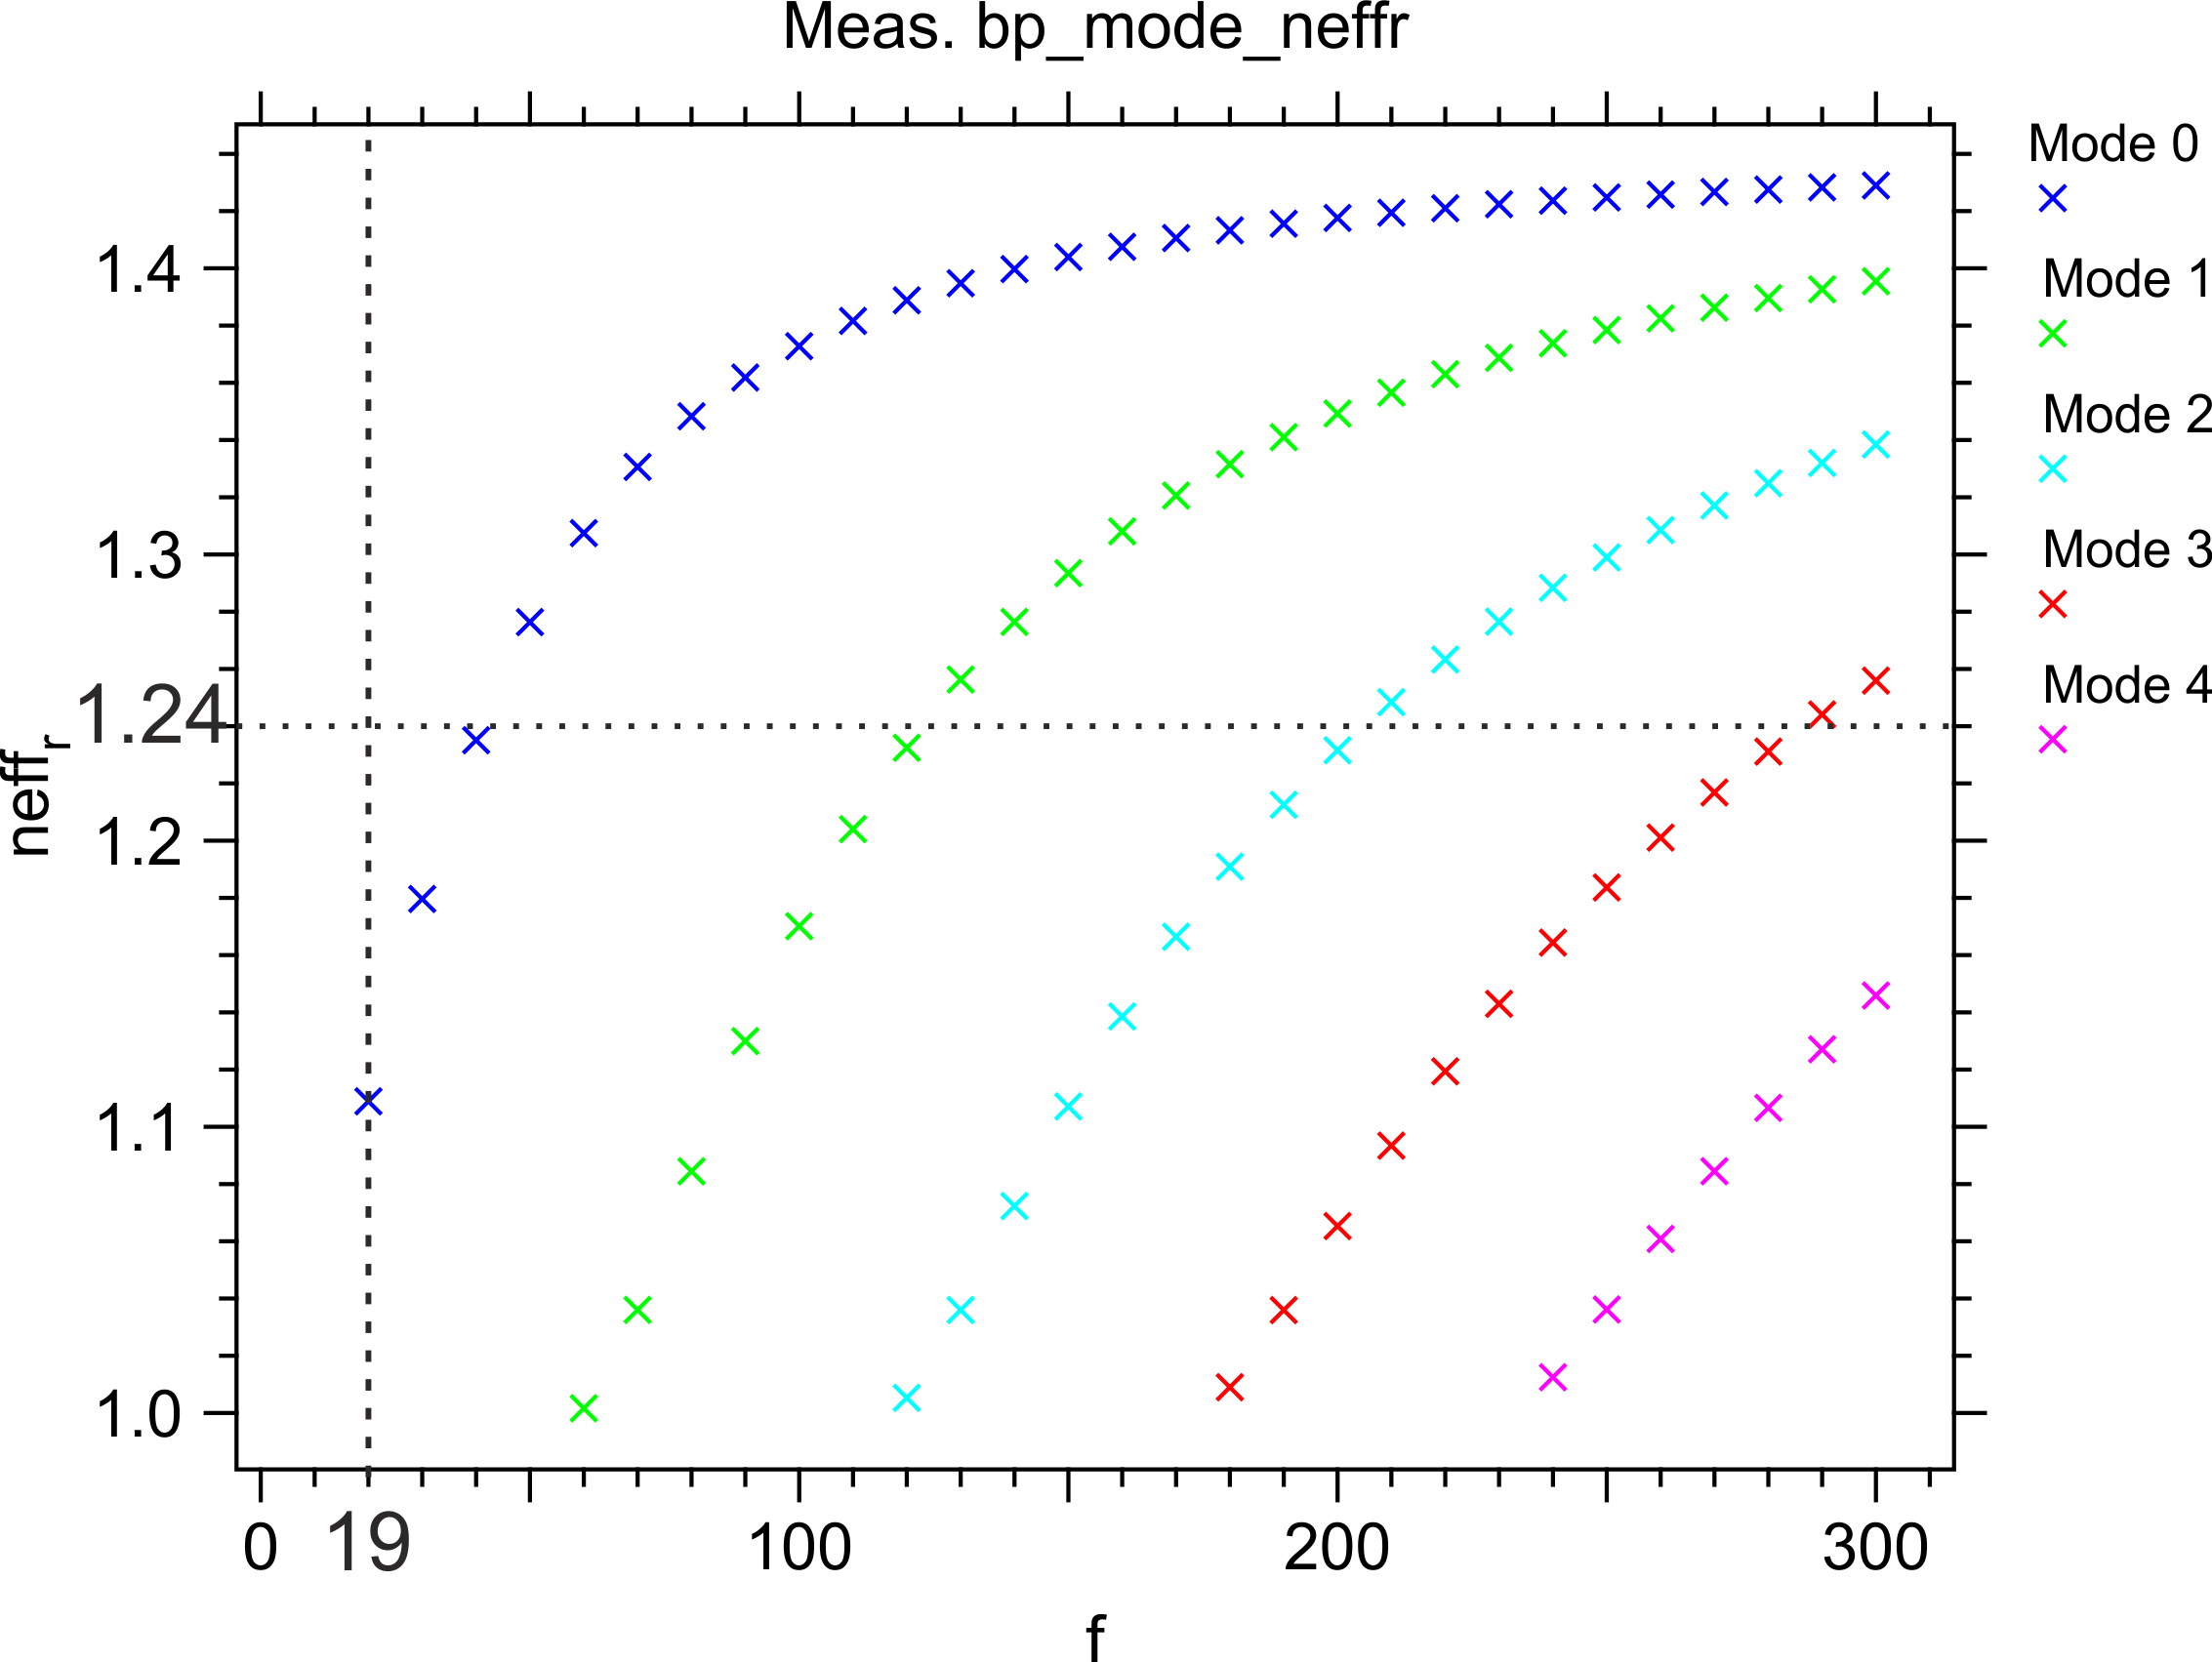
\includegraphics[totalheight=5.5 cm]{Grafiken/TE_neff.png}\label{fig:1_TE_neff}}
	\subfloat[TM]{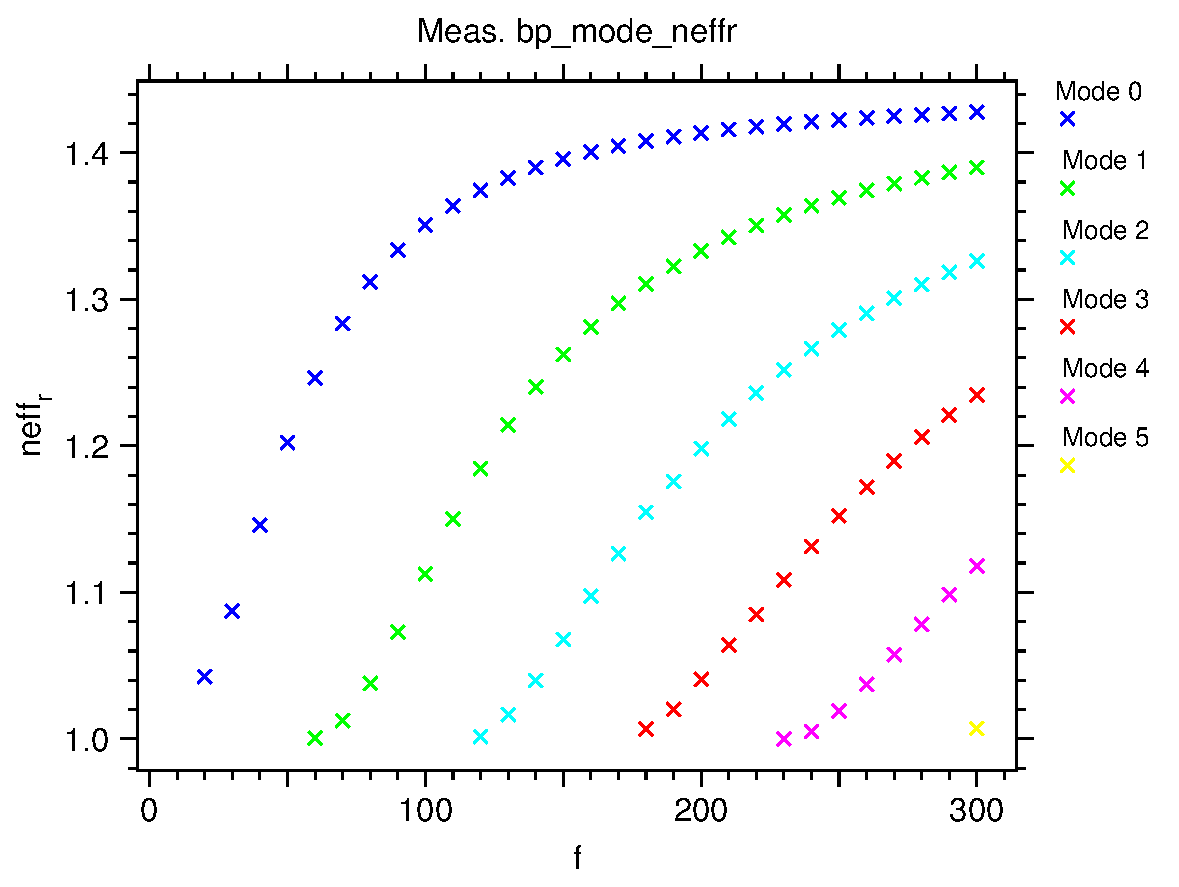
\includegraphics[totalheight=5.5 cm]{Grafiken/scan_TM_neff.pdf} \label{fig:1_TM_neff}}
\caption{Effective refractive indices for different modes and frequencies.}%
\label{fig:1_neff}%
\end{figure}

There is a difference between the effective indices of the TE and the TM modes due the different boundary conditions that both modes fulfill. As seen the TM modes reach lower $n_{eff}$ faster than the TE modes which leads to a worse confinement factor of the TM modes.

For $B = 0$ the normalized frequency is $V = 0$. That means that $f = 0$ as well, and $n_{eff}= 1$. Here both diagrams, \ref{fig:singlemoded} and \ref{fig:1_neff} show the same.

For $B = 0.5$ the normalized frequency is $V\approx\pi/3$.
This corresponds to a frequency of 19~THz and an $n_{eff}$ of 1.24. 
Those values were calculated using equation \eqref{eq:norm_freq} and 
\begin{equation}
B = \frac{n_{eff}^2 - n_2^2}{n_1^2-n_2^2}
\label{eq:}
\end{equation}

As in figure \ref{fig:1_TE_neff} can be seen this values do not match exactly to the measured values.
This difference could be explained by the fact, that figure \ref{fig:singlemoded} is valid for a low index contrast which is not true in our case.

\section{Quadratic single-mode strip waveguide}
\label{sec:task2}

The next step was to simulate a three dimensional strip waveguide in air with a higth and a lenght of 0.356~$\upmu$m and a core refractive index $n$~=~3.03 in air.
The lenght of the waveguide was 100~$\upmu$m.

Figure \ref{fig:2_index} shows the index profile of the waveguide.
% 
% \begin{figure}%
% 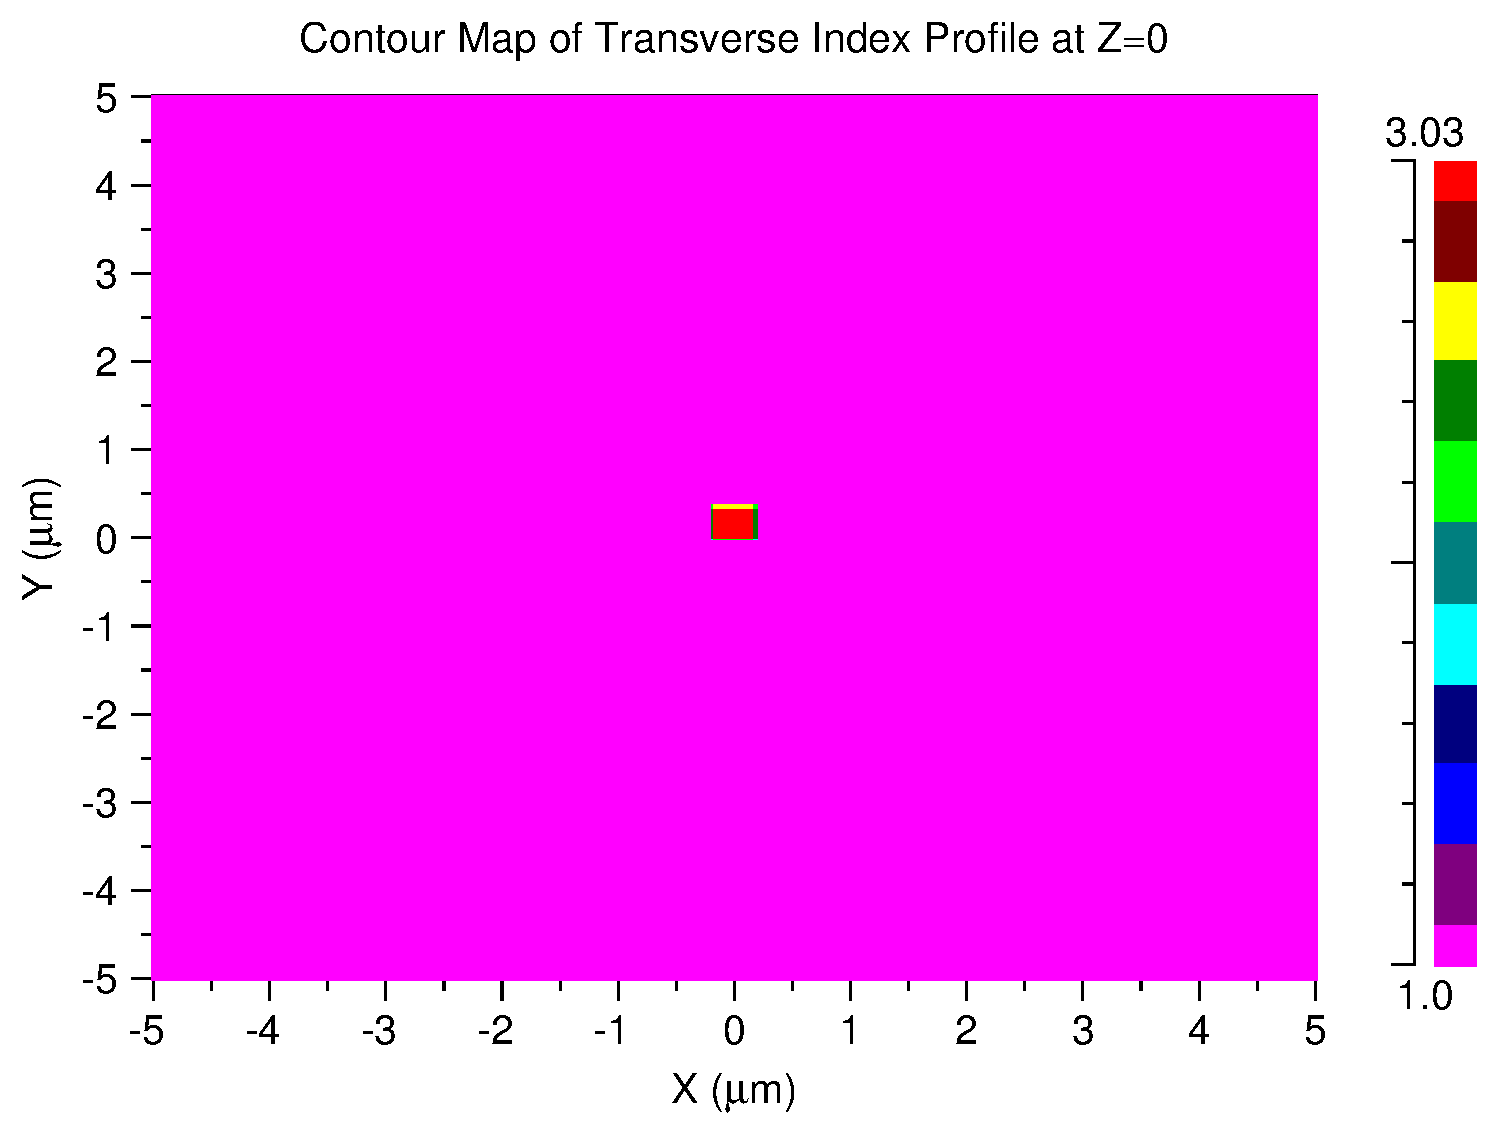
\includegraphics[width=.5\columnwidth]{Grafiken/2_index}%
% \caption{index profile of the quadratic single-mode strip waveguide.}%
% \label{fig:2_index}%
% \end{figure}

\begin{figure}[h]%
\centering
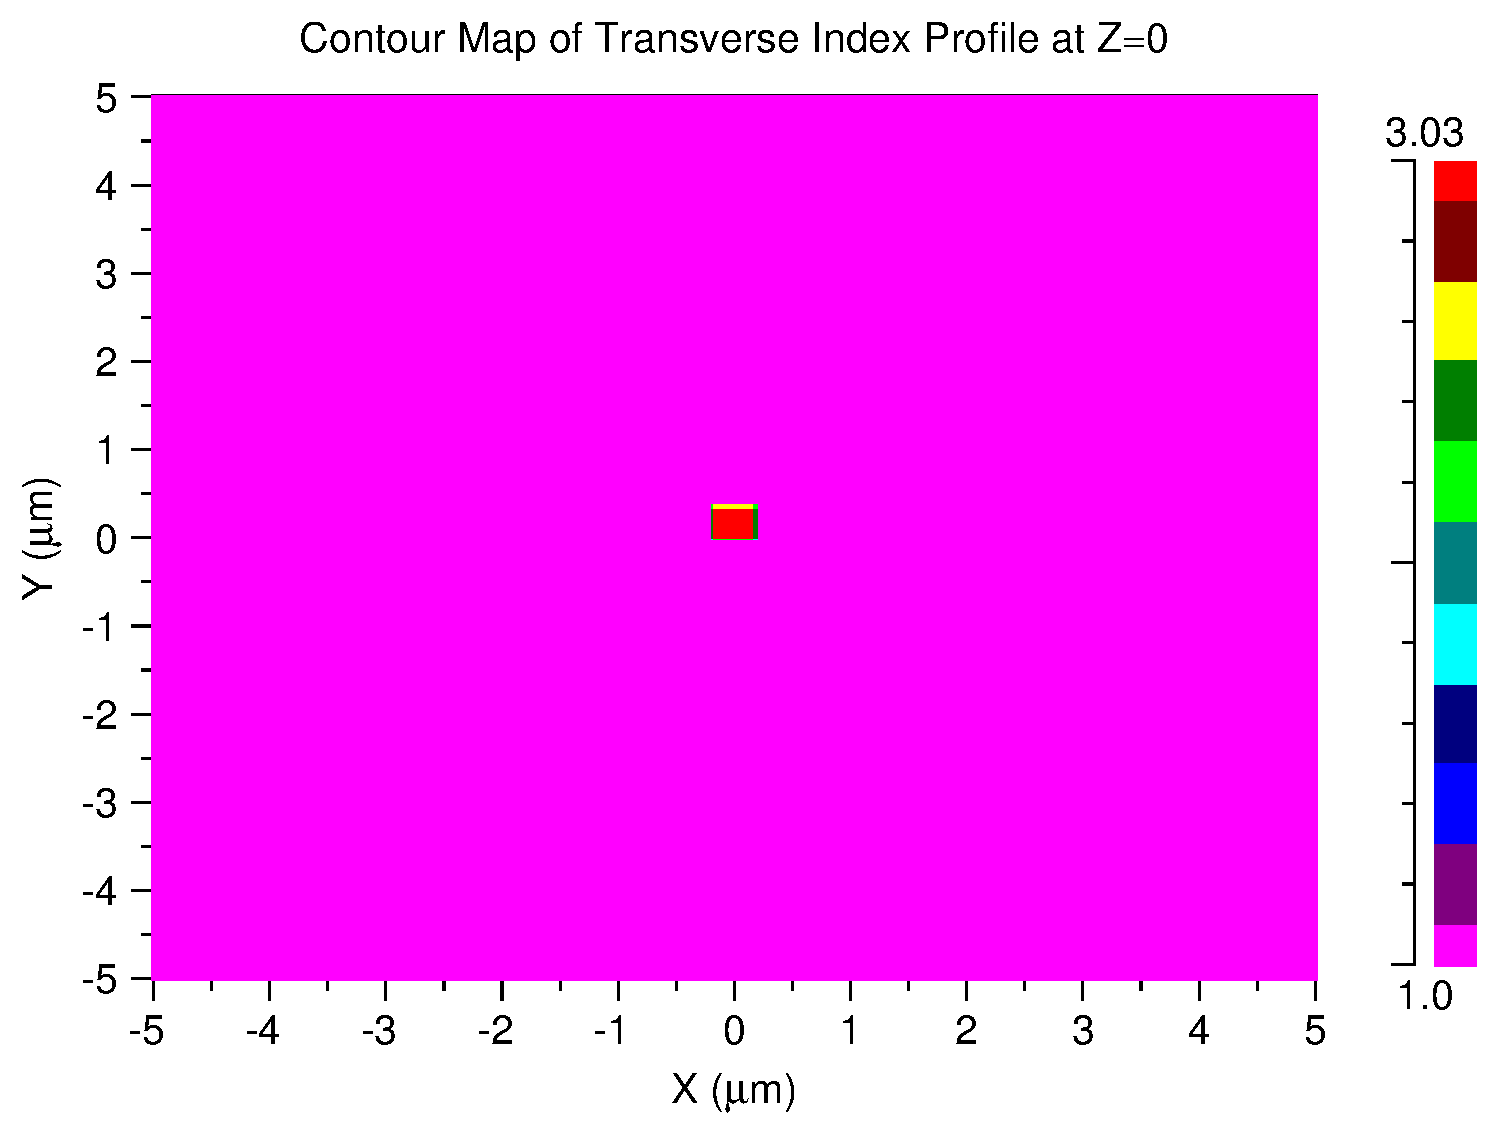
\includegraphics[totalheight=5.5 cm]{Grafiken/2_index.pdf}%
\caption{index profile of the quadratic single-mode strip waveguide.}%
\label{fig:2_index}%
\end{figure}

The excitation of the field is Gaussian and and has an offset in x direction by 0.25 times the width and in y direction by 0.25 times the hight of the waveguide.
For this waveguide all modes wer calculated at a frequency of 200~THz by using the correlation method and a grid size in x/y/z-direction of 0.02/0.02/0.05. 

\begin{figure}[ht]
\centering
%\begin{adjustwidth}{0cm}{0cm}
	\subfloat[HE$_{00}$]{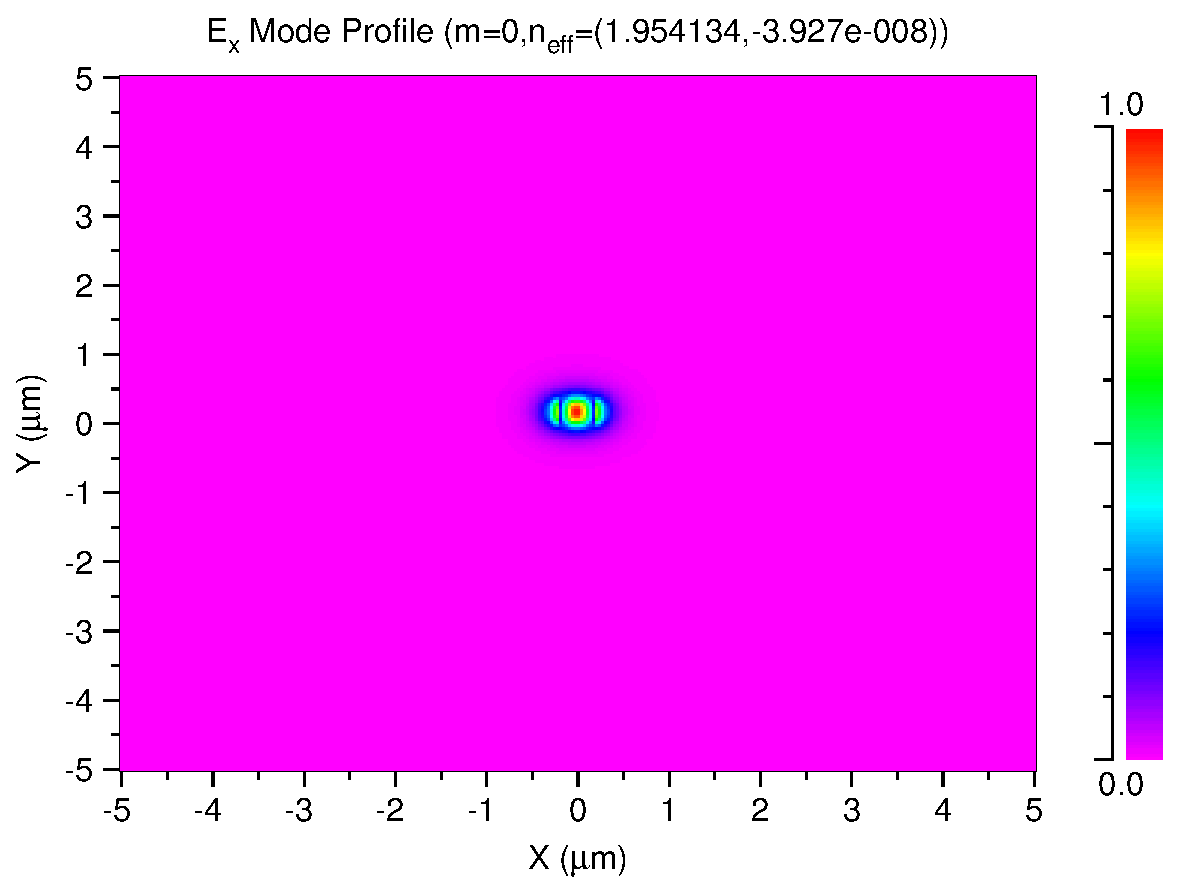
\includegraphics[totalheight=5.5 cm]{Grafiken/2_TE00.pdf}\label{fig:2_TE00}}
	\subfloat[not guided]{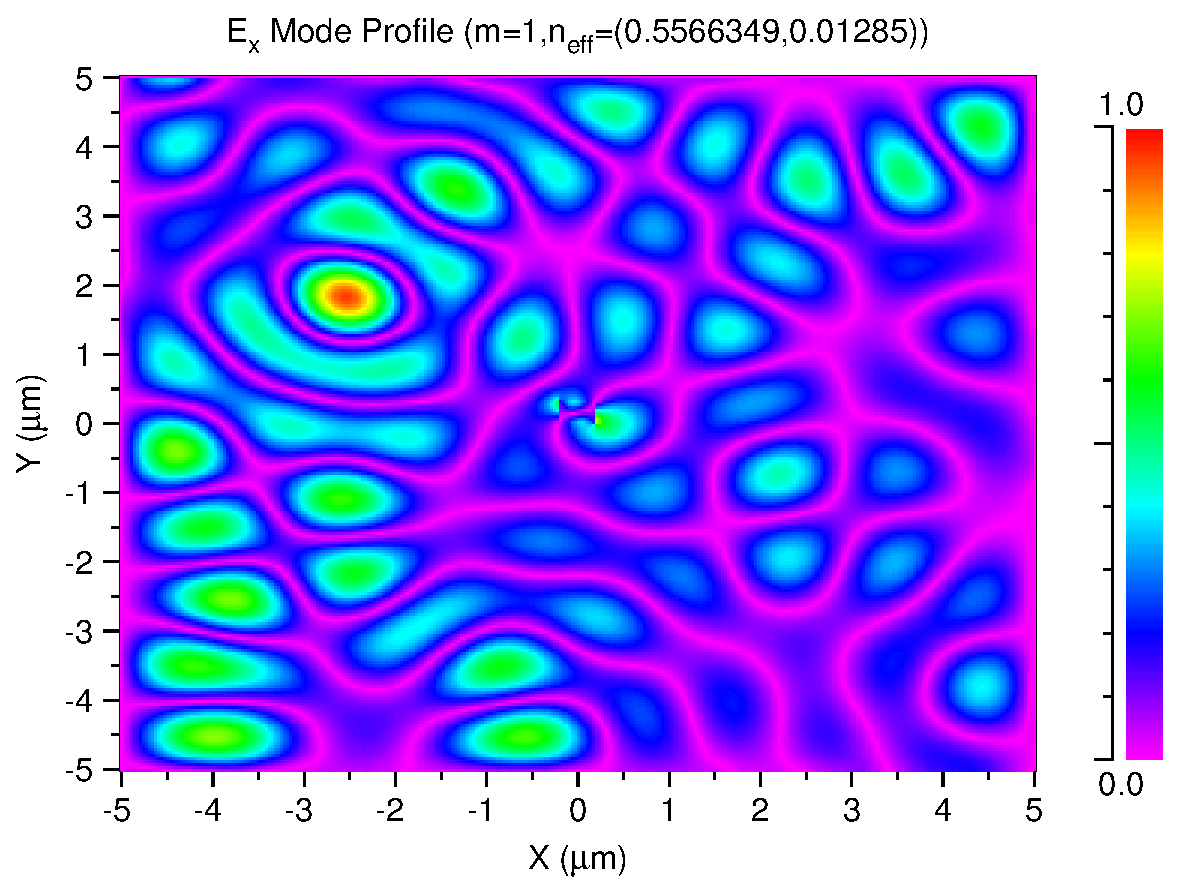
\includegraphics[totalheight=5.5 cm]{Grafiken/2_TE01.pdf} \label{fig:2_TE01}}\\%
	\subfloat[EH$_{00}$]{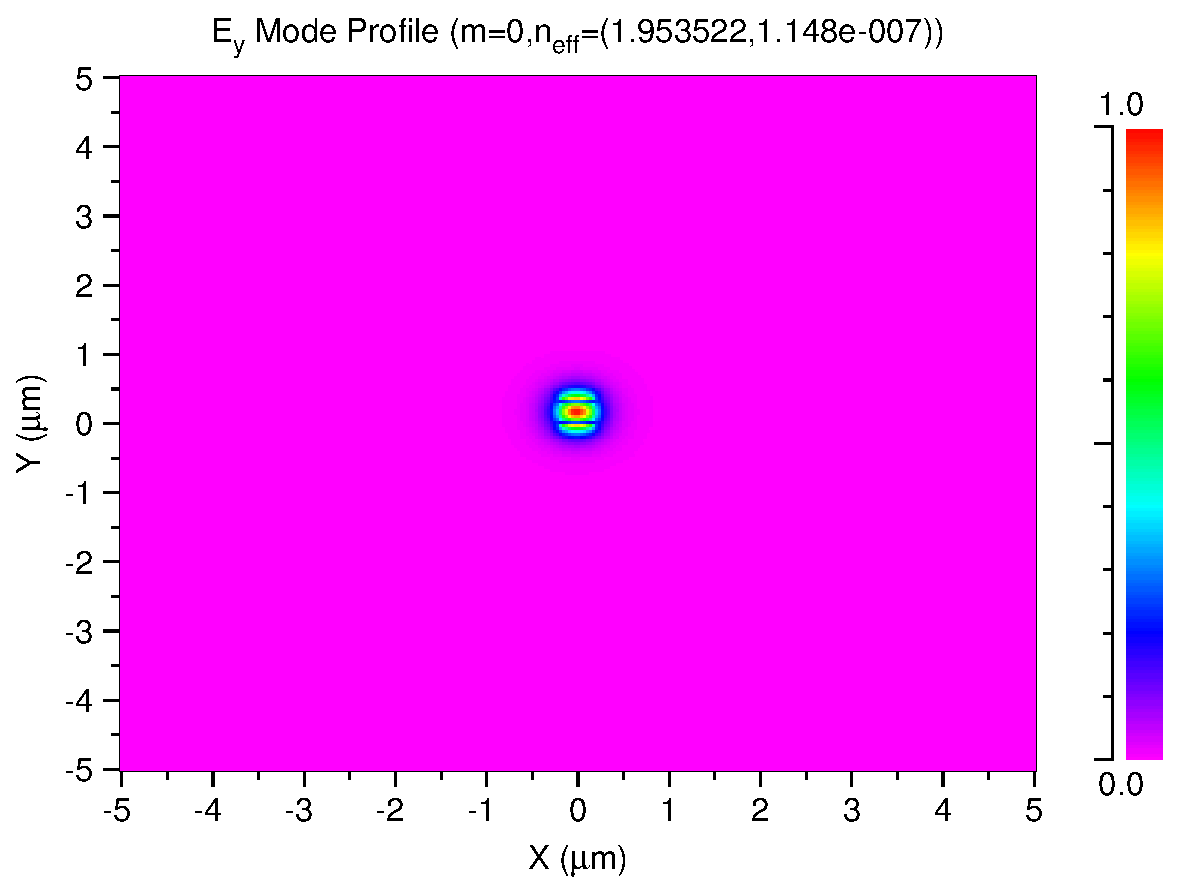
\includegraphics[totalheight=5.5 cm]{Grafiken/2_TM00.pdf}\label{fig:2_TM00}}
%\end{adjustwidth}
\caption{Modes of the quadratic single-mode strip waveguide.}%
\label{fig:2_modes}%
\end{figure}
As figure \ref{fig:2_modes} shows only the ground modes HE$_{00}$ (dominating $\vec{\mathrm{E}}_x$-field: quasi TE) and EH$_{00}$ (dominating $\vec{\mathrm{E}}_y$-field: quasi TM) are guided. The field of the higher quasi TE mode ($m~=~1$) \ref{fig:2_TE01} is not confined to the core and the calculated field makes no sense and since the effective refractive index is below the core index this means that the mode can't be guided as well.

Comparing the HE$_{00}$ (cf. figure \ref{fig:2_TE00}) and the EH$_{00}$ (cf. figure \ref{fig:2_TM00}) modes shows, that the dominating $\vec{\mathrm{E}}$-fields are in different direction. The Field of the HE$_{00}$ is in x-direction and the field of the EH$_{00}$ is in y-direction. Both modes show a discontinuity in the $\vec{\mathrm{E}}$-field that is tangential to the dielectric boundary. This is based on the continuity of the electric displacement field.

Furthermore the field of the EH$_{00}$ shows two larger maxima outside the cure compared to the HE$_{00}$ mode. That means that the field of the HE$_{00}$ is more confined to the core.

For the case that the waveguide is single-moded there are several conditions. As in the preparation (eg. \ref{pre:single-mode}) the normalized frequency $V$ needs to be below $\pi/2$ and $V$ depends on the dimensions of the waveguide, the refractive indices of the materials and the wavelength of the light.
For the given waveguide design the number of modes can be changed by changing the frequency. 
\begin{figure}[ht]%
\centering
%\begin{adjustwidth}{0cm}{0cm}
	\subfloat[TE modes]{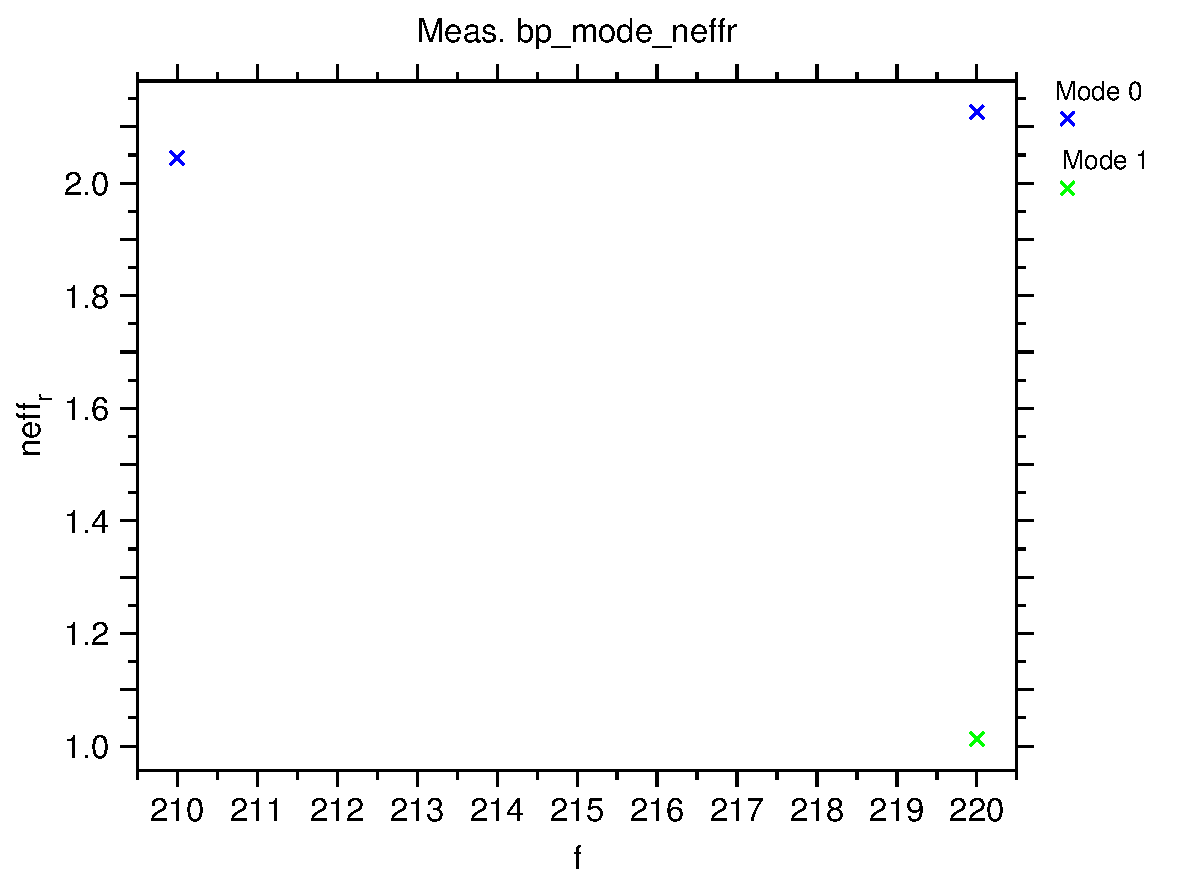
\includegraphics[totalheight=5.5 cm]{Grafiken/2_TE_sweep.pdf}\label{fig:2_TE_sweep}}
	\subfloat[TM modes]{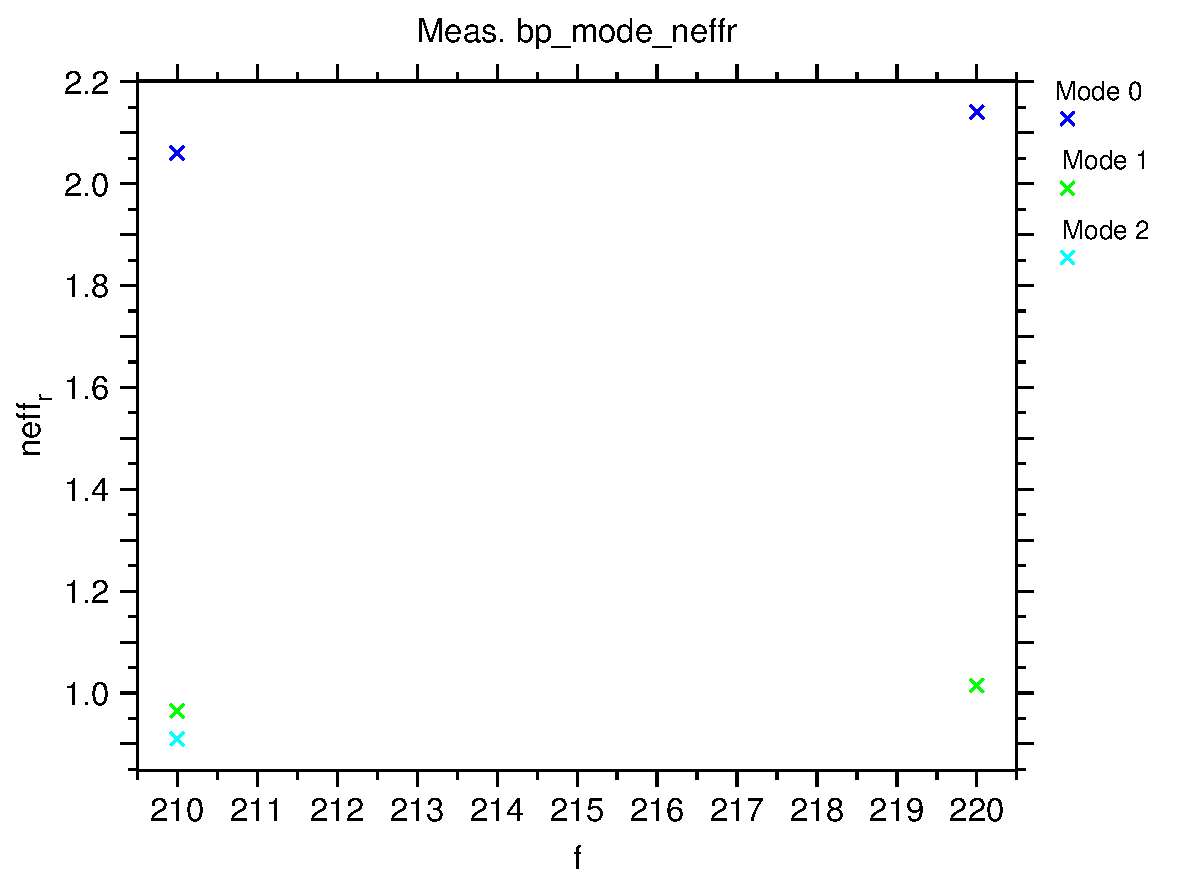
\includegraphics[totalheight=5.5 cm]{Grafiken/2_TM_sweep.pdf} \label{fig:2_TM_sweep}}
\caption{Effective indices for different modes and frequencys}%
\label{fig:2_sweep}%
\end{figure}

Figure \ref{fig:2_sweep} shows the effective indices for different modes and frequencies. In figure \ref{fig:2_TE_sweep} can be seen that the quasi TE-mode for $m~=~1$ is the first time calculated as a guided mode for $f~=~220$~Thz.  Here the effective index is just above 1. For the quasi TM mode it looks nearly the same (cf. figure \ref{fig:2_TM_sweep}). The first of the simulation program calculated quasi TM mode with $m~=~1$ is at 210~THz but the effective index is below 1. That means the mode is not guided at this frequency. For $f = 220$~THz the the quasi-TM mode for $m$~=~1 is guided as well.
This means that for a frequency of $f = 220$~THz the waveguide becomes multimode.



\section{Design of a SOI strip waveguide}

\begin{figure}[h]%
\centering
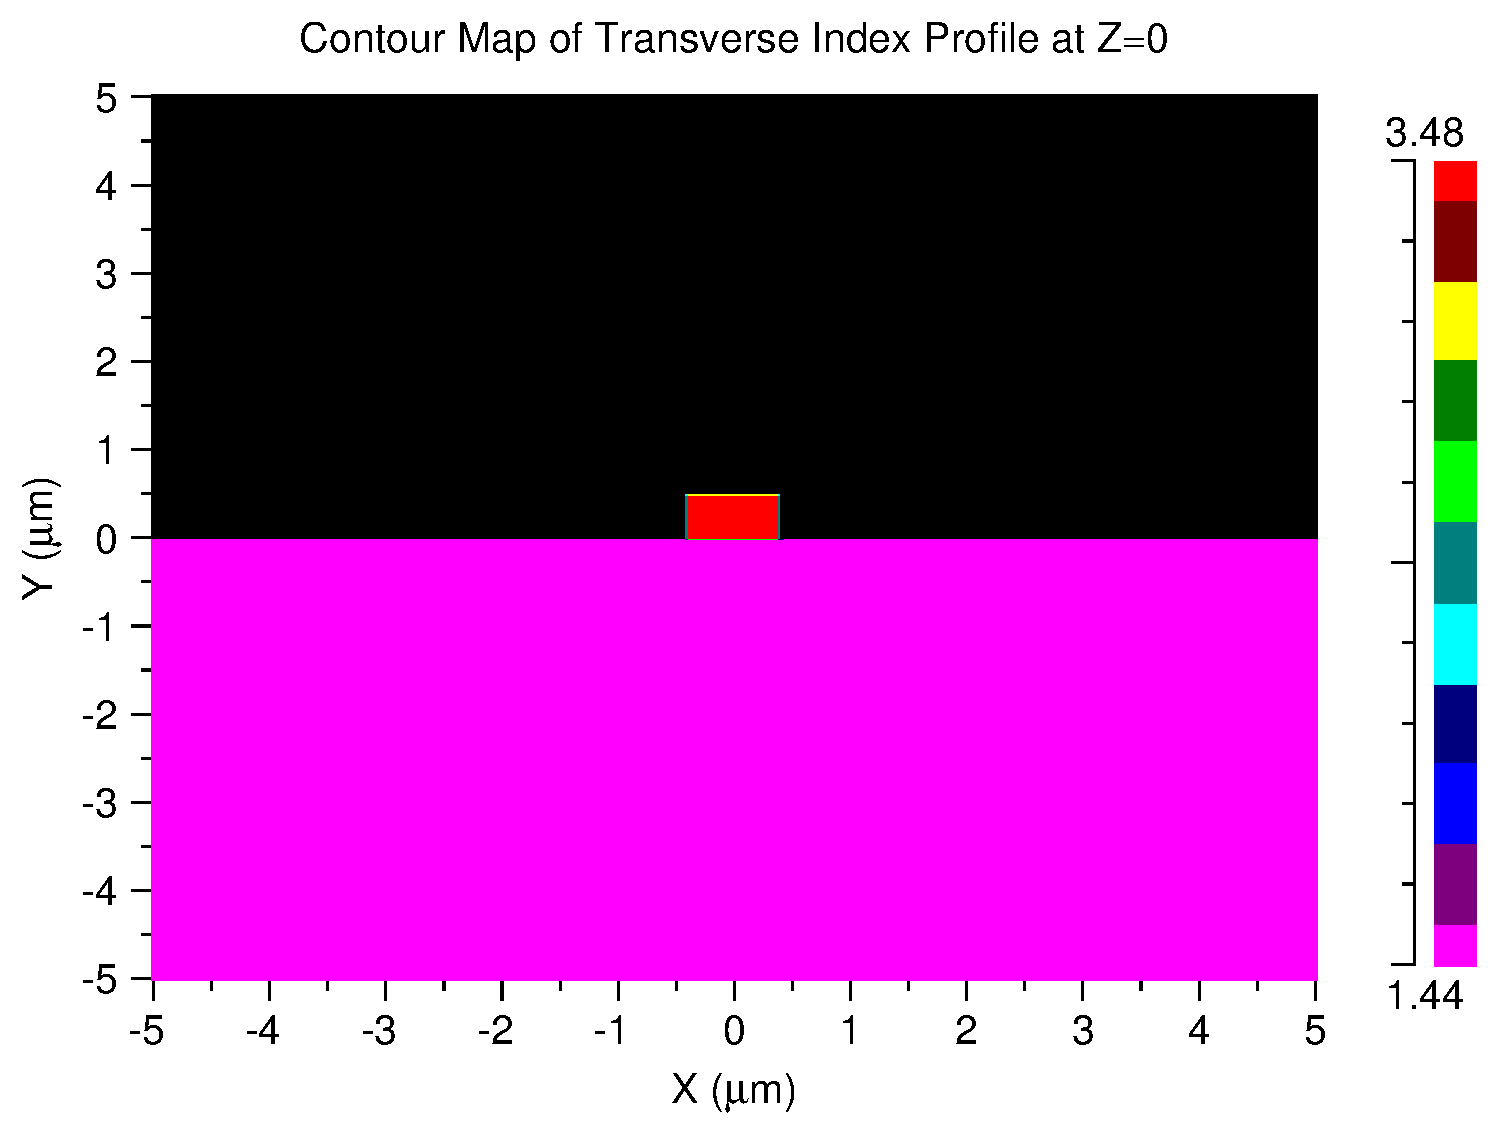
\includegraphics[totalheight=5.5 cm]{Grafiken/3_index.pdf}%
\caption{index profile of the SOI strip waveguide}%
\label{fig:index_profile_3}%
\end{figure}
In the third task a silicon on insulator (SOI) strip waveguide of the length of $100~\upmu$m is simulated. The waveguide consists of a silicon core ($n=3.48$) with the height $h=0.7~\upmu$m and a width of $w=0.8~\upmu$m. This core is placed on a glass substrate ($n=1.44$). Above and on both sides of the waveguide there is air. This index profile is shown in \ref{fig:index_profile_3}. The gaussian exitation is shifted $0.25\cdot w$ in x-direction and $0.25\cdot h$ in y-direction, like in the task \ref{sec:task2}.

Next the TE and TM modes for $\lambda = 1.55~\upmu$m were calculated by using the correlation method. The field distribution of the calculated modes is shown in the figures \ref{fig:3TE} and \ref{fig:3TM}. The figures were named according to the nomenclature in the OWS lecture notes. The calculated modes \ref{fig:ng}, \ref{fig:ng2} and \ref{fig:ng3} are not guided because the effective index is lower than the refractive index in the substrate. The modes \ref{fig:HE20} and \ref{fig:EH02} are guided, but heavily damped because the field is badly confined to the core. Thus the propagation of these modes can be neglegted.

%% VORSICHT!!!!! %%
%% die Label sin noch falsch, dh passen nicht zur benennung.

\begin{figure}%
\centering
	\subfloat[HE$_{00}$  ]{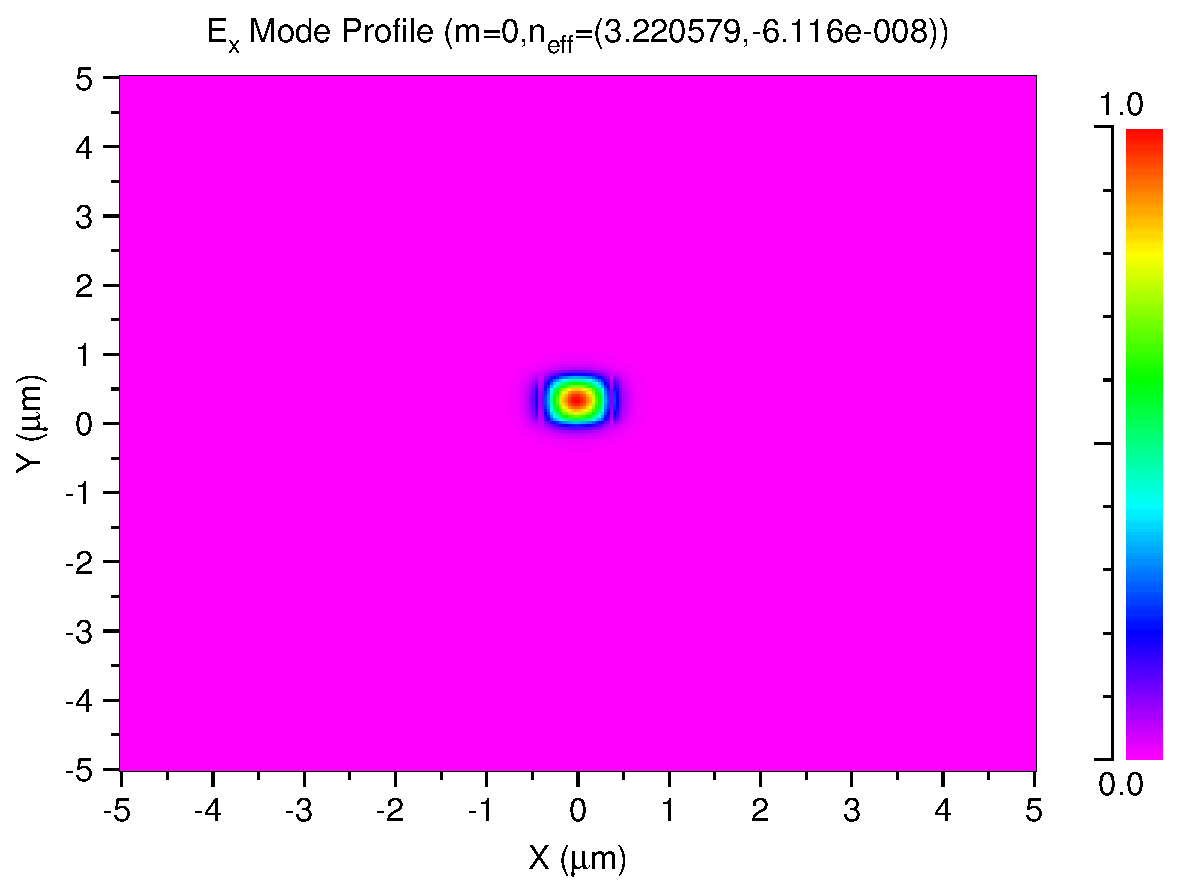
\includegraphics[totalheight=5 cm]{Grafiken/A3_TE_00.pdf}\label{fig:HE00}}
	\subfloat[HE$_{01}$  ]{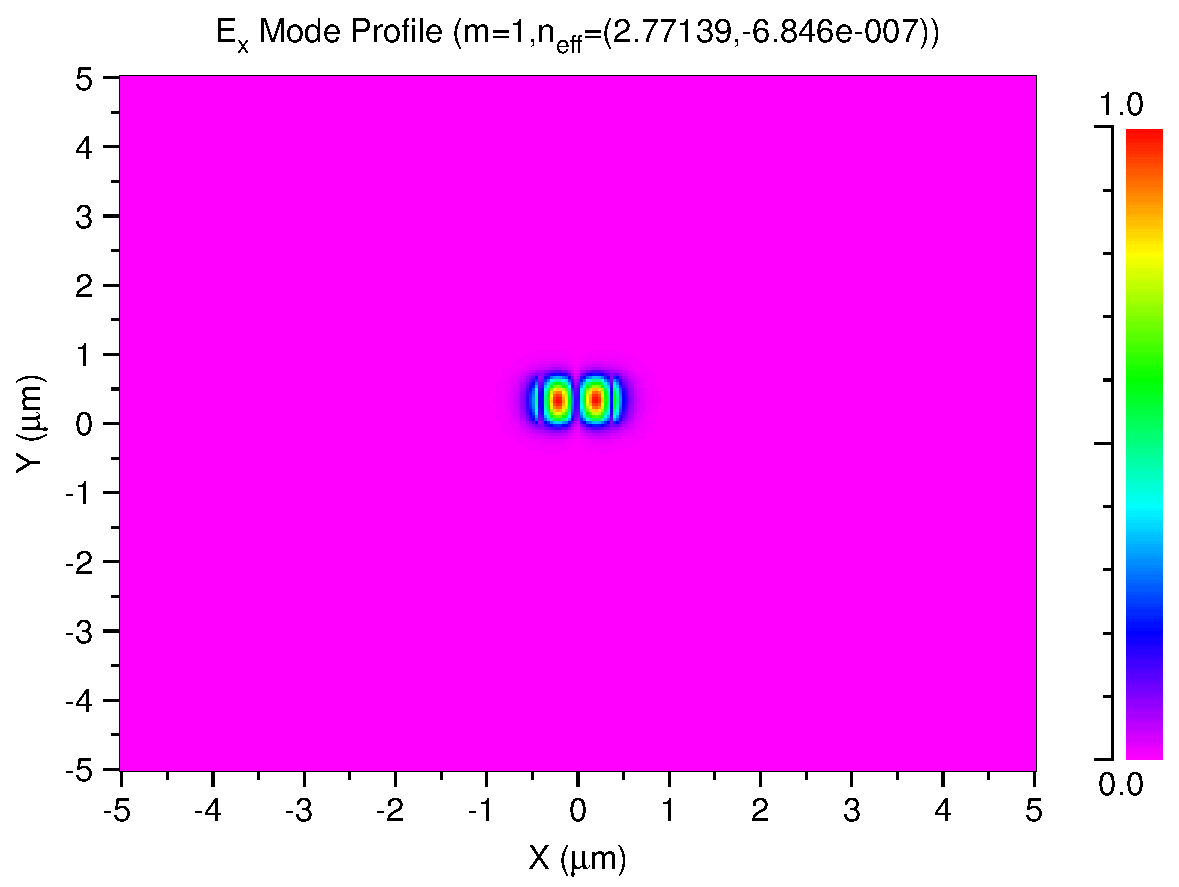
\includegraphics[totalheight=5 cm]{Grafiken/A3_TE_01.pdf} \label{fig:HE10}}\\%
	\subfloat[HE$_{11}$  ]{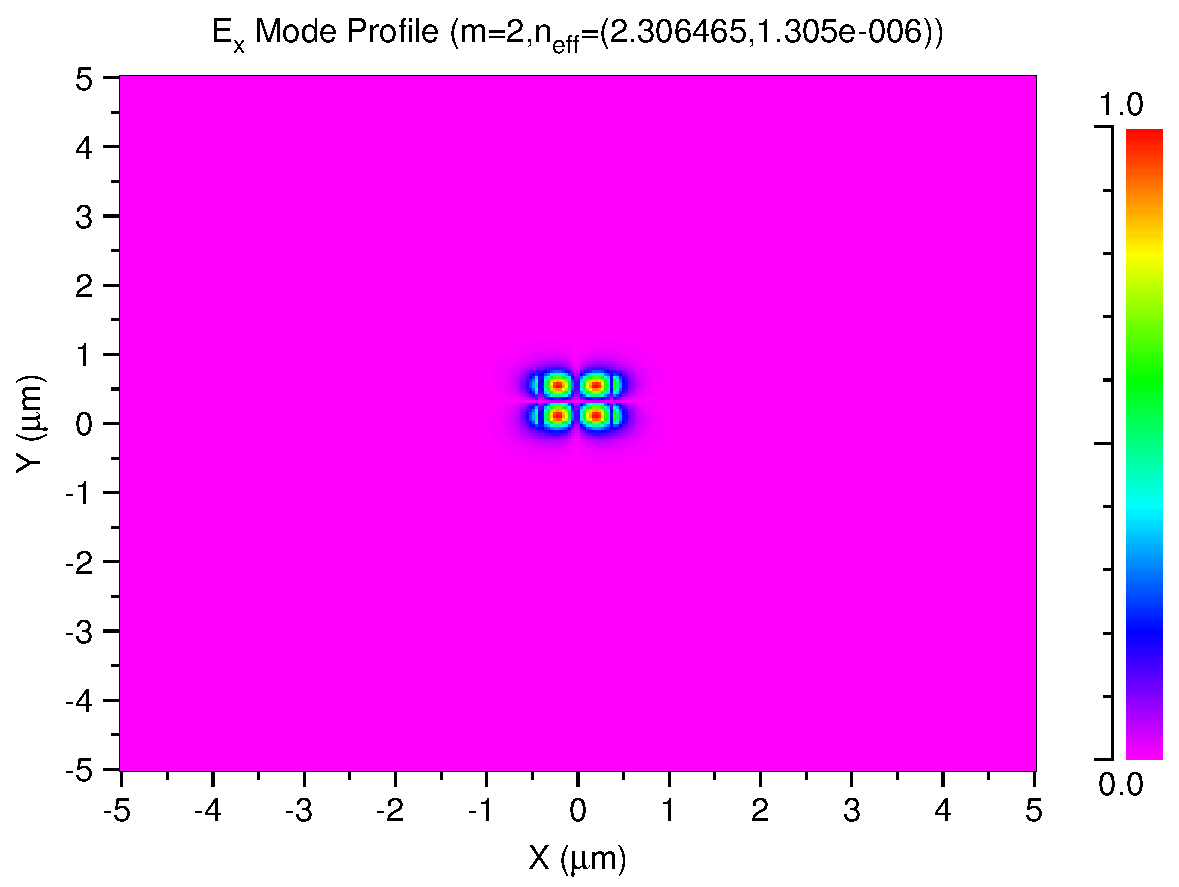
\includegraphics[totalheight=5 cm]{Grafiken/A3_TE_02.pdf}\label{fig:HE11}}
	\subfloat[HE$_{20}$  ]{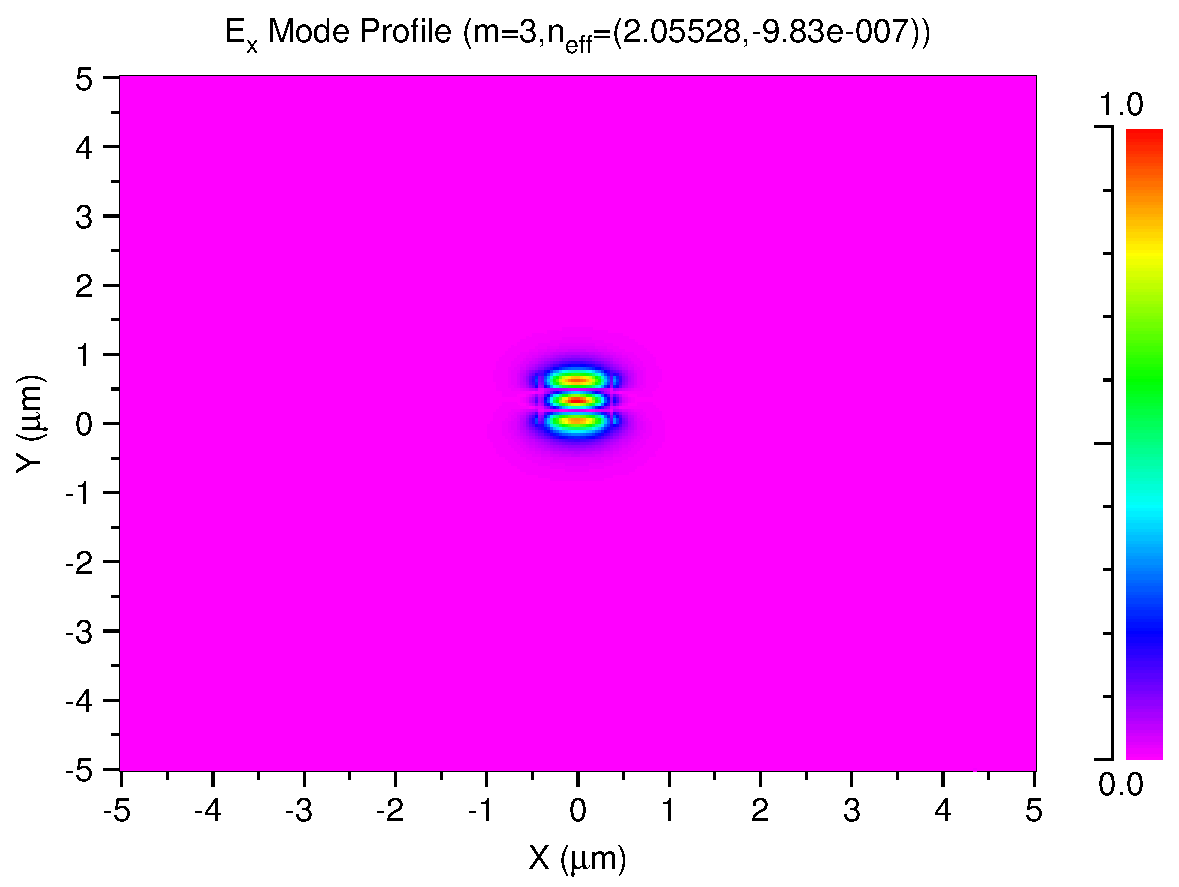
\includegraphics[totalheight=5 cm]{Grafiken/A3_TE_03.pdf} \label{fig:HE02}}\\
        \subfloat[HE$_{02}$  ]{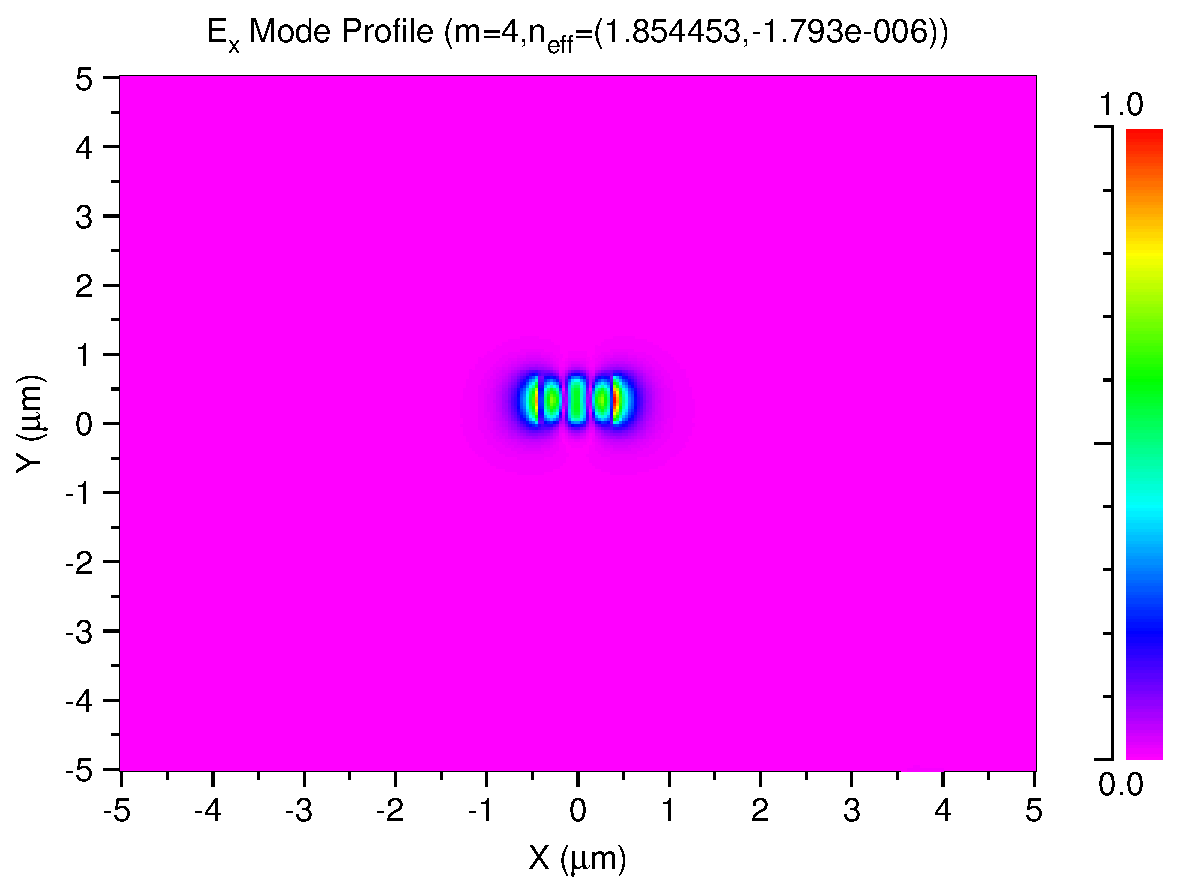
\includegraphics[totalheight=5 cm]{Grafiken/A3_TE_04.pdf}\label{fig:HE20}}
	\subfloat[not guided  ]{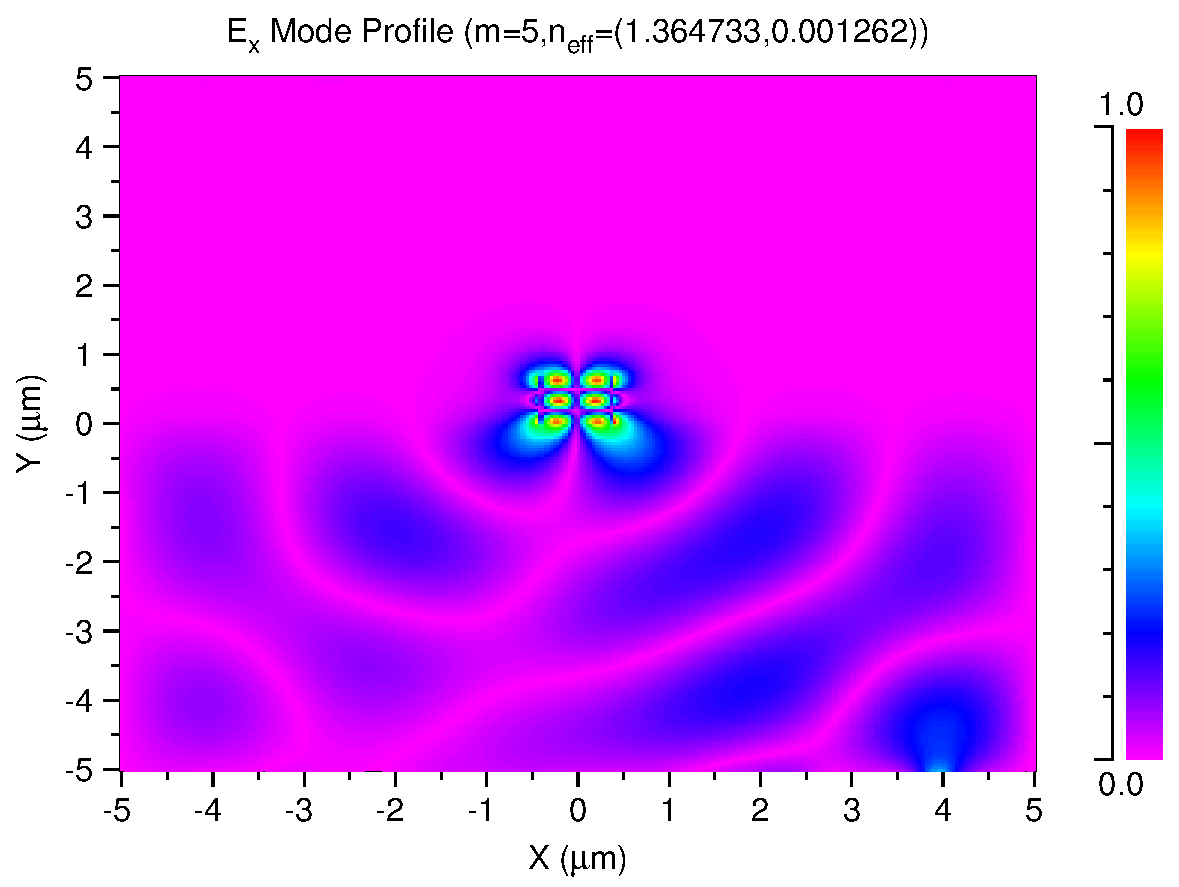
\includegraphics[totalheight=5 cm]{Grafiken/A3_TE_05.pdf} \label{fig:ng}}\\
	\subfloat[not guided  ]{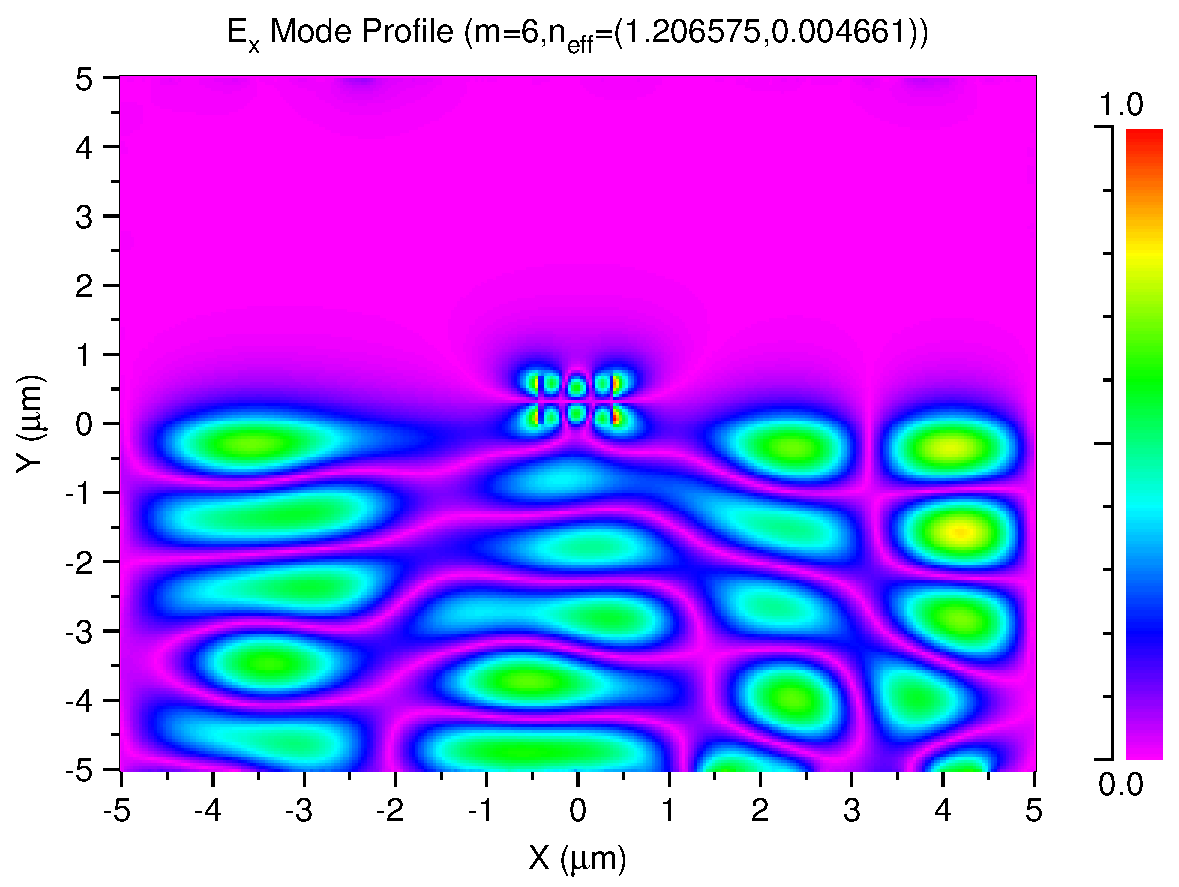
\includegraphics[totalheight=5 cm]{Grafiken/A3_TE_06.pdf}\label{fig:ng2}}
\caption{}%
\label{fig:3TE}%
\end{figure}

\begin{figure}%
\centering
	\subfloat[EH$_{00}$  ]{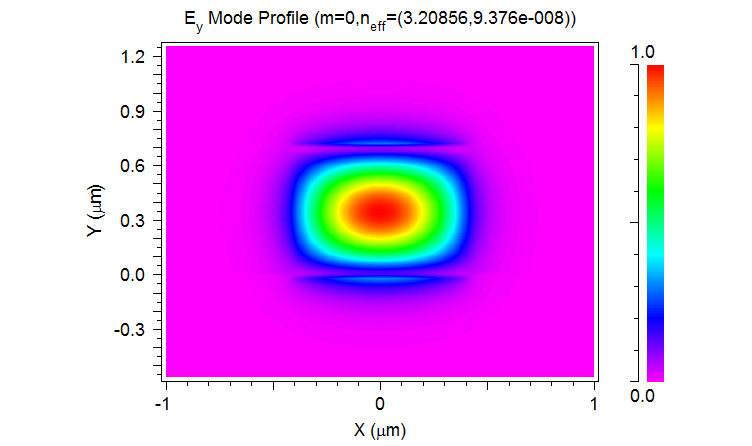
\includegraphics[totalheight=5 cm]{Grafiken/SOI_TM_mode_00.png}\label{fig:EH00}}
	\subfloat[EH$_{01}$  ]{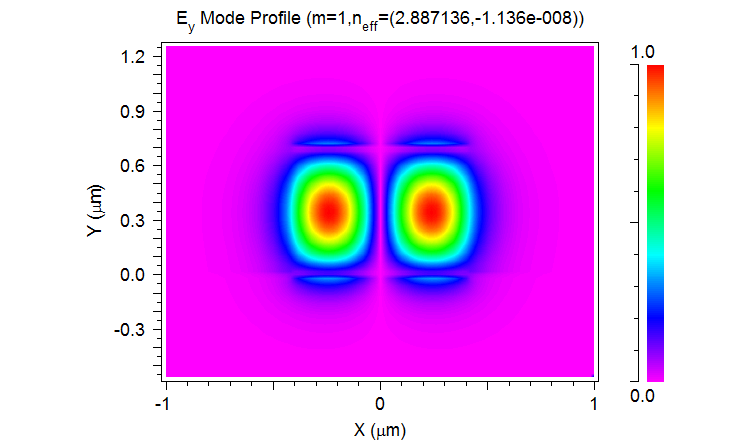
\includegraphics[totalheight=5 cm]{Grafiken/SOI_TM_mode_01.png} \label{fig:EH10}}\\%
	\subfloat[EH$_{10}$  ]{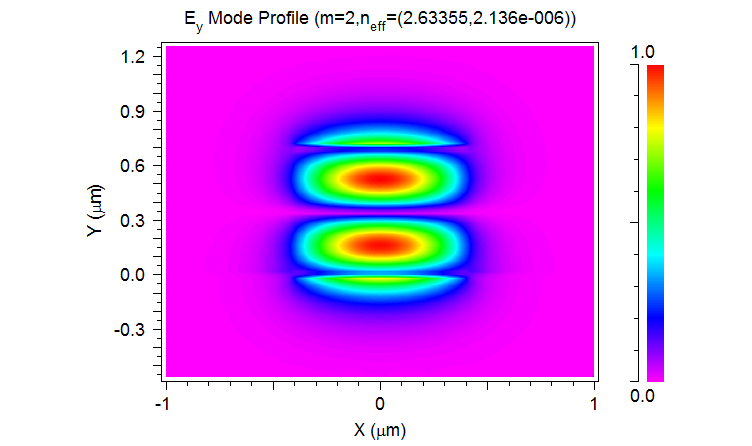
\includegraphics[totalheight=5 cm]{Grafiken/SOI_TM_mode_02.png}\label{fig:EH01}}
	\subfloat[EH$_{02}$  ]{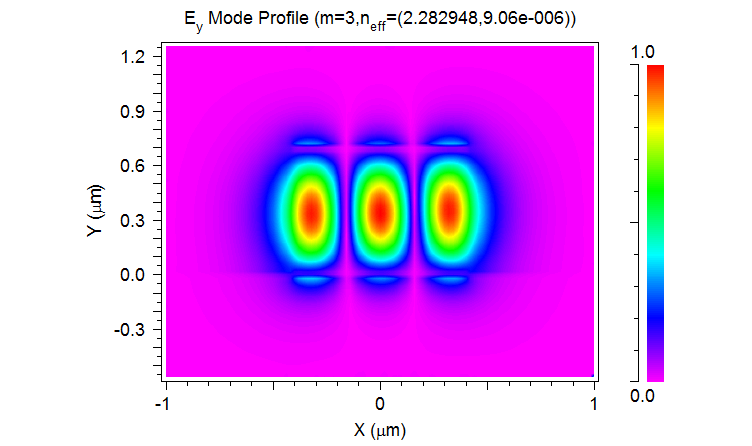
\includegraphics[totalheight=5 cm]{Grafiken/SOI_TM_mode_03.png} \label{fig:EH20}}\\
        \subfloat[EH$_{11}$  ]{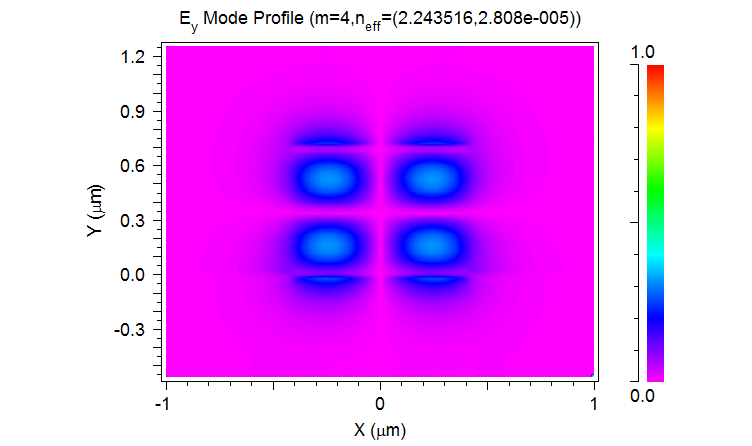
\includegraphics[totalheight=5 cm]{Grafiken/SOI_TM_mode_04.png}\label{fig:EH11}}
	\subfloat[EH$_{20}$  ]{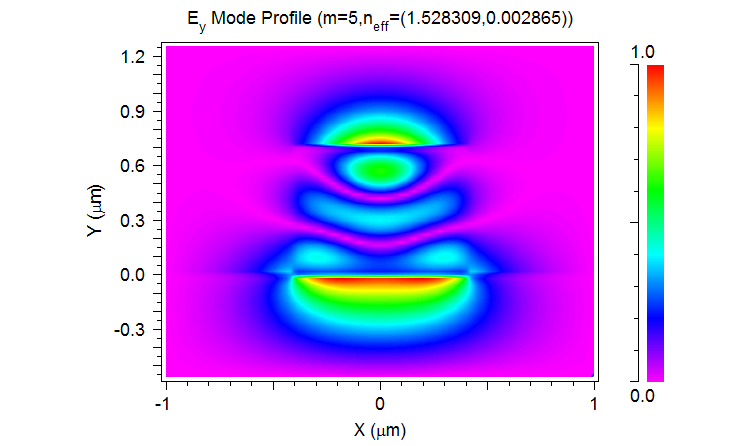
\includegraphics[totalheight=5 cm]{Grafiken/SOI_TM_mode_05.png} \label{fig:EH02}}\\
	\subfloat[not guided  ]{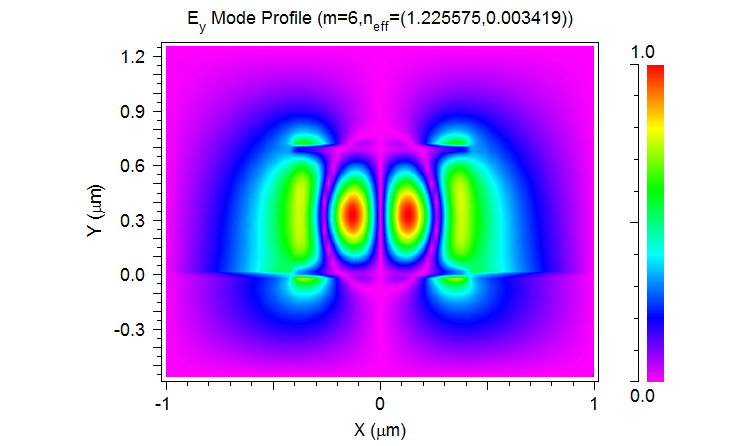
\includegraphics[totalheight=5 cm]{Grafiken/SOI_TM_mode_06.png}\label{fig:ng3}}
\caption{}%
\label{fig:3TE}%
\end{figure}


At the last the dimensions of the waveguide were varied that only one mode is guided for a wavelength of about $1.55~\upmu$m in the strip waveguide. A single mode waveguide could be achieved for a height of 0.2~$\upmu$m and a width of 0.55~$\upmu$m. For this dimensions, TE01 and TM01 are not guided anymore.
